\documentclass[11pt]{jreport}
\usepackage{wuse_thesis}
\usepackage{indentfirst}
\usepackage{color}
\usepackage{url}	% \url{}コマンド用.URLを表示する際に便利
\newcommand{\todo}[1]{\colorbox{yellow}{{\bf TODO}:}{\color{red} {\textbf{[#1]}}}} 	
\usepackage{graphicx}  % ←graphicx.styを用いてEPSを取り込む場合有効にする
\usepackage{tabularx}
\usepackage{multirow}
\usepackage[hang,small,bf]{caption}
\usepackage[subrefformat=parens]{subcaption}
\usepackage{here}
\usepackage{amsmath}

% 他のパッケージ・スタイルを使う場合には適宜追加	

%%%%%%%%%%%%%%%%%%%%%%%%%%%%%%%%%%%%%%%%%%%%%%%%%%%%%%%%%%%%%%%%%%%%%%%%

%%
%% 主に表紙を作成するための情報
%%

%%  タイトル(修論の場合は英語表記も指定)
\title{オブジェクトの動作に基づく\\
	Scratch作品の直感的検索手法}

%\title{オブジェクト動作経路の時系列解析に基づくビジュアルプログラム作品検索の試み}       

%\etitle{Test\\Test\\Test}

%%  著者名(修論の場合は英語表記も指定)
\author{福地 ユキ}
%\eauthor{Akinori Ihara}

%% 卒業論文・修士論文(以下のどちらかを選択)
\bachelar	% 卒業論文(4年生用)
%\master  	% 修士論文(M2用)

%%  学科・クラスタ
\department{システム工}
%\department{デザイン情報}
%\department{デザイン科学}

%%  学生番号
\studentid{60236238}

%%  卒業年度
\gyear{2021}		% 提出年が2022年なら,2021年度

%%  論文提出日
\date{2022年2月15日}	% 修士の場合は月(2021年2月)までとし,英語表記も指定
%\edate{February 2021}	% 修士の場合,こちら(英語表記)も有効化

%%%%%%%%%%%%%%%%%%%%%%%%%%%%%%%%%%%%%%%%%%%%%%%%%%%%%%%%%%%%%%%%%%%%%%%%

\begin{document}

\maketitle

%%
%%  概要
%%
\begin{abstract}

ビジュアルプログラミング言語は,視覚的に表現された命令処理を操作することで
プログラムを実装可能なプログラミング言語である.
ビジュアルプログラミング学習サービスの1つであるScratchでは,
ユーザが制作したプログラム作品をオンラインサービス上に公開可能である.
Scratchのオンラインサービス上には,多数のユーザが制作した膨大な数の作品が公開されており,
ユーザは他者の作品を参照することで多様な実装方法を学習する.
参照する他者の作品を探し出すためにキーワード検索を行うが,ユーザがイメージする動作を言語化することは難しく,
動作に関するキーワードをタイトルや説明文に含まない作品は検索不可能であるため,
ユーザがイメージする動作を含む作品を検索することは容易ではない.
キーワードによる検索ではなく,マウスを用いた描画等によって動作のイメージを入力とする
直感的な検索を実現することで,ユーザがイメージする動作を含む作品の検索を容易にできると考える.

本研究では,動作のイメージを入力とする,オブジェクトの動作に基づくScratch作品の直感的検索手法を提案する.
入力と検索対象の各動作の類似度合いを測るために,
2つの時系列データの距離を算出する動的時間伸縮法を用いる.類似動作を抽出可能な距離を明らかにするために,
13,437件の公開作品を対象に入力を行い,距離算出結果の分析を行なった.
分析では,入力との距離が異なる複数の動作を被験者に提示し,被験者全員が類似していない
と判断する値よりも近い距離を,類似動作を抽出可能な距離とした.
結果は,〜.\todo{結果を載せる}

本研究は,動作のイメージを入力とするScratch作品の直感的検索手法を提案することで
検索を容易にし,他者の作品を参照することによる実装方法の学習が促進されることを期待する.

\end{abstract}

%%  目次
\tableofcontents

%%  図目次 (図目次をいれたければ以下のコメントをはずす)
%\listoffigures

%%  表目次 (表目次をいれたければ以下のコメントをはずす)
%\listoftables

\newpage
\pagenumbering{arabic}	% 以降のページ番号を算用数字に

%%%%%%%%%%%%%%%%%%%%%%%%%%%%%%%%%%%%%%%%%%%%%%%%%%%%%%%%%%%%%%%%%%%%%%%%

%%
%%  本文はここから
%%


\chapter{はじめに}

初等教育からのプログラミング必修化に伴い,プログラミング教育が進められている.
特に,テキストの入力ではなく,視覚的に表現された命令処理の操作でプログラムを実装する
ビジュアルプログラミング言語が利用されている.
ビジュアルプログラミング言語は,直感的にプログラムを実装可能なことや,
視覚的に表現されたプログラムの理解が容易であること,
テキストベースのプログラミング言語で障壁となるテキスト入力の間違いが発生しないことなどから,
プログラミング初学者が取り組みやすい言語となっている.

ビジュアルプログラミング言語を用いた代表的な学習サービスScratch\footnote{ \url{https://scratch.mit.edu/}}は,
ユーザが制作した作品をタイトル・説明文を添えてオンラインサービス上に公開している.
2022年1月時点で8,300万以上の人がScratchに登録しており,
オンラインサービス上に9.400万件以上の作品を公開している
\footnote{\url{https://scratch.mit.edu/statistics/}}.
Scratchのユーザは,オンラインサービス上の他者の作品を参照することで多様な実装方法を学習する\cite{spfa}.
参照する作品を探し出すために,ユーザは作品のタイトルと説明文を対象としたキーワード検索を行う.
しかし,イメージする動作を検索キーワードへ変換することはユーザにとって難しく,
動作に関するキーワードをタイトルや説明文に含まない作品は検索結果に表示されないため,
ユーザのイメージを含む作品の検索は容易ではない\cite{wild}.
作品検索が容易ではないという課題は,他者の作品を参照する学習の障壁になると示唆する.
キーワードによる検索ではなく,動作のイメージを入力とするScratch作品の直感的な検索を実現することで,
ユーザのイメージに類似する動作を含む作品の検索を容易にできる.
検索を行う際,ユーザにとって類似する動作の基準を決定することが本研究の課題となる.

本論文では,マウスを用いた描画によって動作のイメージを入力することで,
動作の言語化を必要としない,簡単な操作で完結するScratch作品の直感的検索手法を提案する.
入力と検索対象動作の類似度合いを測るために,2つの時系列データの距離を算出する動的時間伸縮法を用いる.
類似動作を抽出可能な距離を明らかにするために,13,437件の公開作品を対象に入力を行い,
距離算出結果から入力と動作の類似性を評価する分析を行う.
動作のイメージを入力とするScratch作品の直感的検索手法を実現することで
作品検索を容易にし,他者の作品を参照する学習の支援を期待する.

続く2章では,Scratchにおけるプログラム作品検索の背景と課題について述べる.
3章では提案手法について述べ,
4章では入力と動作の類似性を評価する分析とその結果について述べる.
5章では分析結果を考察し,最後に6章でまとめを述べる.


\chapter{ビジュアルプログラミング言語Scratchにおけるプログラム作品検索}

\section{Scratch}
\label{scratchsetumei}
Scratch\footnote{ \url{https://scratch.mit.edu/}}は,MITメディアラボが開発する
ビジュアルプログラミング言語の1つである.
Scratchでは「10歩動かす」「15度回す」などの命令処理がブロックで視覚的に表現されており,
ユーザは複数のブロックを組み合わせることで,画面上のオブジェクトを動かす作品を制作する.
Scratchで制作される作品の種類は,ゲームやストーリー,アニメーションなど多岐に渡る\cite{wild}.
Scratchは,直感的にプログラムを実装可能なことや,プログラムの理解が容易であること,
テキストベースのプログラミング言語で障壁となるテキスト入力の間違いによる構文エラーが発生しないことなどから,
プログラミング初学者が取り組みやすいプログラミング言語となっている.
従来研究では,Scratchを用いた学習がプログラミング学習に有効であり,テキストベースのプログラミング言語への
移行を容易にすることを明らかにしている\cite{blocktotext}\cite{blockandbeyond}.

図\ref{scratchdisplay}は,Scratch3.0における作品制作画面を示す.
作品は主に「ブロック」「スクリプト」「スプライト」の3つの要素で構成されている.

\begin{itemize}
    \item ブロック: 命令処理を1つのブロックで表現する.
    図\ref{scratchdisplay}の(1)に示す複数のブロックを繋ぎ合わせて使用する.
    命令処理の種類によって形状や色が異なる.表\ref{blockshape}は形状の種類と性質,
    表\ref{blockcolor}は色の種類と性質を示す.
    \item スクリプト: 複数のブロックを組み合わせて制作したひとまとまりのプログラムである.
    スクリプトはイベント駆動型であり,図\ref{scratchdisplay}の(2)に示すスクリプトの例では,
    スペースキーが押された際にプログラムが実行される.
    \item スプライト: キャラクター等の画像のオブジェクトである.
    スプライトに対してスクリプトを制作することで,プログラムをスプライトに実行させる.
    作品制作の初期画面では,図\ref{scratchdisplay}の(3)に示すCatがあらかじめ配置されている.
    ユーザはスプライトを複数配置することができ,Scratchが標準で用意している画像や,
    ユーザが創作した画像をスプライトとして使用可能である.
\end{itemize}

図\ref{scratchdisplay}に示す例は,スペースキーが押された際にCatのスプライトが
「こんにちは!」と発言し,その後進行方向に10歩移動する動作を10回繰り返す作品である.

Scratchで制作した作品は,図\ref{scratchonline}の(1)に示すタイトルと
図\ref{scratchonline}の(2)に示す説明文を添えてオンラインサービス上に公開することができる.
2022年1月時点で,8,300万人以上の人がScratchに登録しており,
オンラインサービス上に9.400万件以上の作品を公開している
\footnote{\url{https://scratch.mit.edu/statistics/}}.
他者の公開作品のプログラムを閲覧できるため,ユーザは他者の作品を参照することで
多様な実装方法を学習できる\cite{spfa}.

\begin{figure}[H]
    \centering
    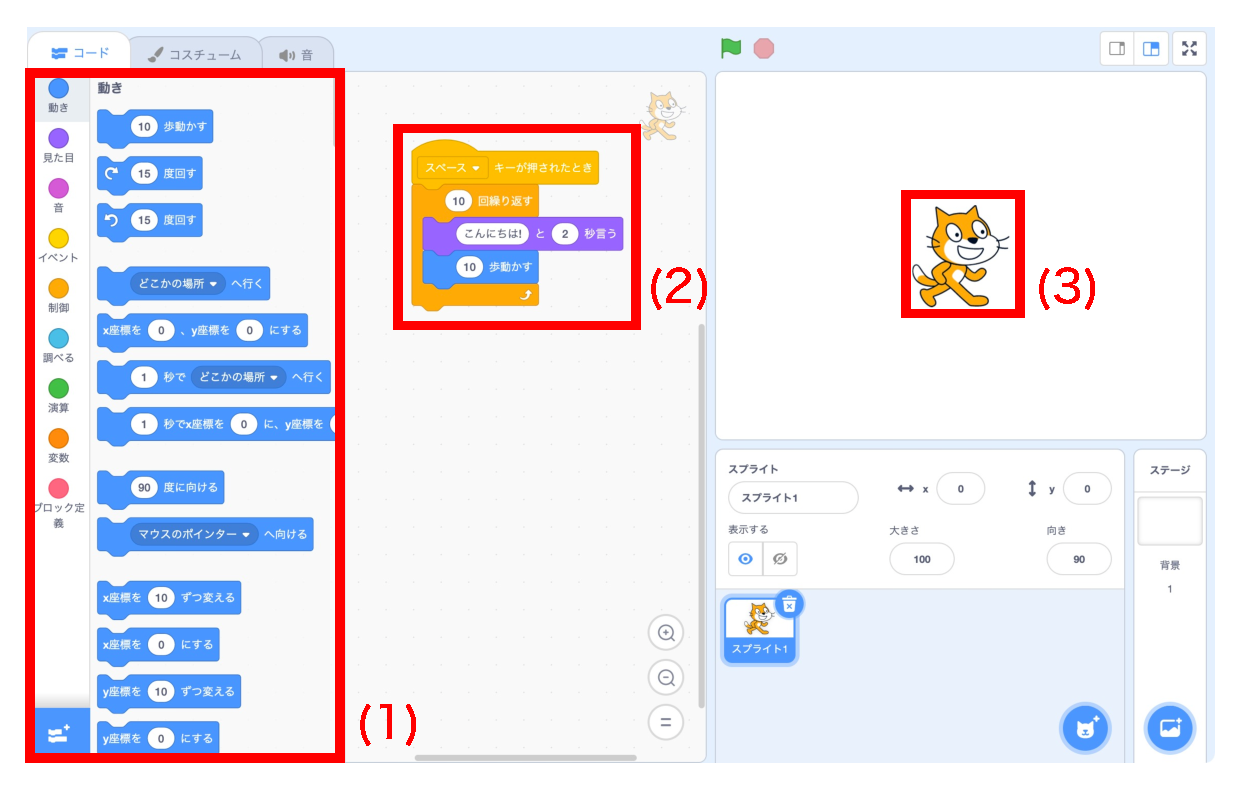
\includegraphics[width=12cm]{scratch_display.eps}
    \caption{Scratchの作品制作画面}
    \label{scratchdisplay}
\end{figure}

\begin{figure}[H]
    \centering
    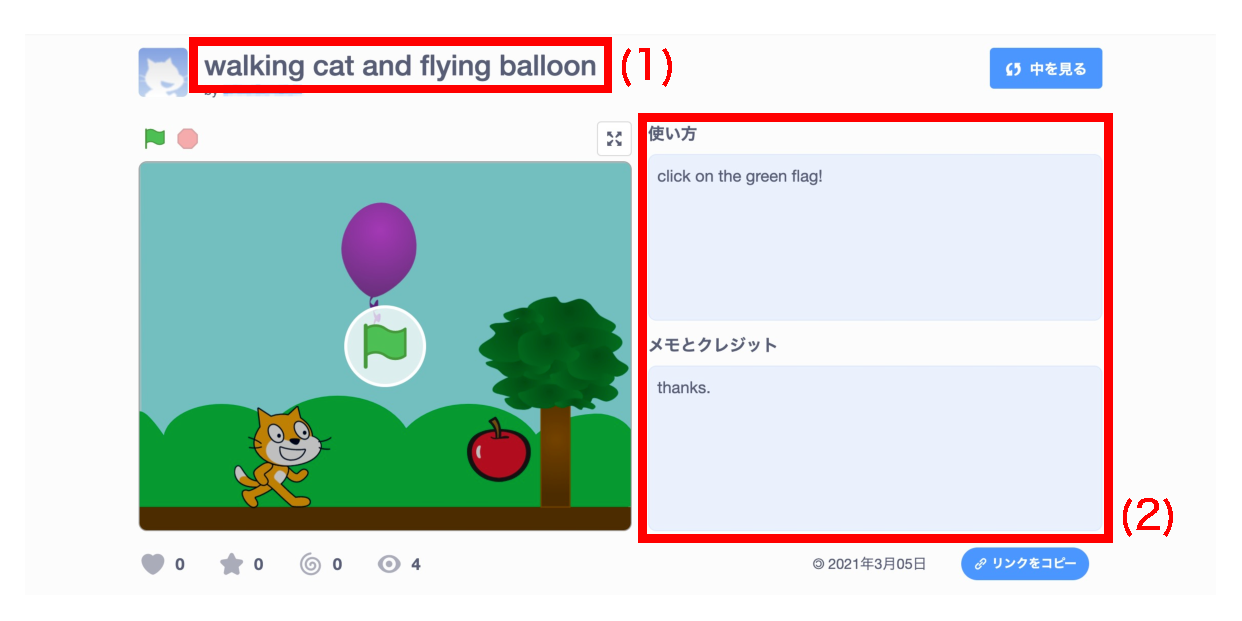
\includegraphics[width=15cm]{scratch_online.eps}
    \caption{公開したScratch作品画面}
    \label{scratchonline}
\end{figure}

\begin{table}[H]
  \caption{ブロックの形状と名前と性質}
  \label{blockshape}
  \centering
  \begin{tabularx}{\textwidth}{l|l|X}
    \hline
    \multicolumn{1}{c|}{ブロックの形状} & \multicolumn{1}{c|}{名前} & \multicolumn{1}{c}{性質} \\
    \hline \hline
    \begin{minipage}{30mm}
      \centering
      \scalebox{0.8}{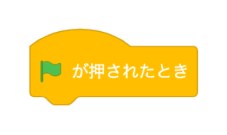
\includegraphics{press_greenflag.eps}}
    \end{minipage} & ハットブロック &  スクリプトの処理を開始するブロック \\
    \hline
    \begin{minipage}{30mm}
      \centering
      \scalebox{0.8}{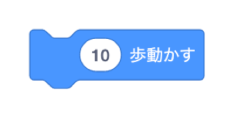
\includegraphics{walk.eps}}
    \end{minipage} & スタックブロック &  記述された命令を実行するブロック \\
    \hline
    \begin{minipage}{30mm}
      \centering
      \scalebox{0.8}{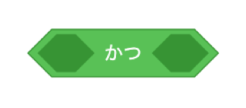
\includegraphics{and.eps}}
    \end{minipage} & 真偽ブロック &  真偽値を保持し,他のブロックの引数となるブロック \\
    \hline
    \begin{minipage}{30mm}
      \centering
      \scalebox{0.8}{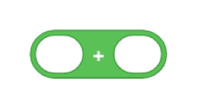
\includegraphics{add.eps}}
    \end{minipage} & 値ブロック &  値を保持し,他のブロックの引数となるブロック \\
    \hline
    \begin{minipage}{30mm}
      \centering
      \scalebox{0.8}{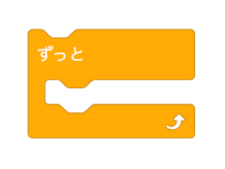
\includegraphics{forever.eps}}
    \end{minipage} & C型ブロック &  間にあるブロックに対して,条件分岐や繰り返しを実行するブロック \\
    \hline
     \begin{minipage}{30mm}
      \centering
      \scalebox{0.8}{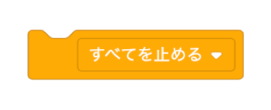
\includegraphics{stop.eps}}
    \end{minipage} & キャップブロック &  スクリプトの処理を停止するブロック \\
    \hline
  \end{tabularx}
\end{table}

\begin{table}[H]
  \caption{ブロックの色と名前と性質}
  \label{blockcolor}
  \centering
  \begin{tabularx}{\textwidth}{l|l|X}
    \hline
    \multicolumn{1}{c|}{ブロックの色} & \multicolumn{1}{c|}{名前} & \multicolumn{1}{c}{性質} \\
    \hline \hline
    \begin{minipage}{30mm}
      \centering
      \scalebox{0.8}{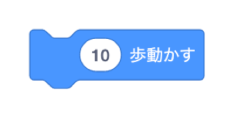
\includegraphics{walk.eps}}
    \end{minipage} & 動きブロック & スプライトを動かすブロック \\
    \hline
    \begin{minipage}{30mm}
      \centering
      \scalebox{0.8}{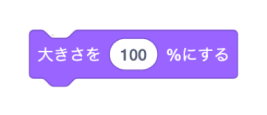
\includegraphics{size.eps}}
    \end{minipage} & 見た目ブロック &  スプライトの見た目を制御するブロック \\
    \hline
    \begin{minipage}{30mm}
      \centering
      \scalebox{0.8}{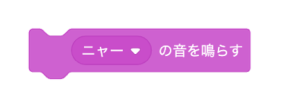
\includegraphics{sound.eps}}
    \end{minipage} & 音ブロック &  BGMやSEをいった音を制御するブロック \\
    \hline
    \begin{minipage}{30mm}
      \centering
      \scalebox{0.8}{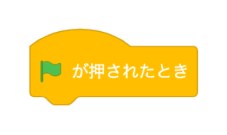
\includegraphics{press_greenflag.eps}}
    \end{minipage} & イベントブロック &  スクリプト実行のトリガーとなるブロック \\
    \hline
    \begin{minipage}{30mm}
      \centering
      \scalebox{0.8}{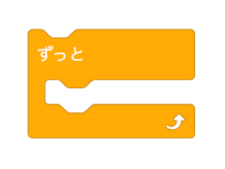
\includegraphics{forever.eps}}
    \end{minipage} & 制御ブロック &  スクリプトを制御するブロック \\
    \hline
     \begin{minipage}{30mm}
      \centering
      \scalebox{0.8}{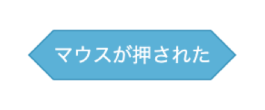
\includegraphics{press_mouse.eps}}
    \end{minipage} & 調べるブロック &  スプライトや操作などの状態を調べるブロック \\
    \hline
    \begin{minipage}{30mm}
      \centering
      \scalebox{0.8}{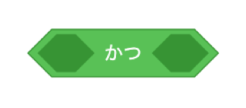
\includegraphics{and.eps}}
    \end{minipage} & 演算ブロック &  数値や論理,文字列に対する演算を行うブロック \\
    \hline
    \begin{minipage}{30mm}
      \centering
      \scalebox{0.8}{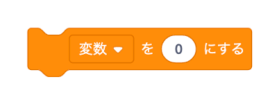
\includegraphics{variable.eps}}
    \end{minipage} & 変数ブロック &  変数とリストを扱うブロック \\
    \hline
    \begin{minipage}{30mm}
      \centering
      \scalebox{0.8}{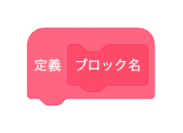
\includegraphics{define.eps}}
    \end{minipage} & ブロック定義ブロック &  メソッドを定義するブロック \\
    \hline
  \end{tabularx}
\end{table}

\section{Scratch作品の検索}

ユーザは,Scratchオンラインサービス上に公開されている膨大な数の
作品を参照することで多様な実装方法を学習することができる\cite{spfa}.
参照する作品を探し出すために,ユーザは作品のタイトルと説明文を対象としたキーワード検索を行う.
C言語やJavaをはじめとするテキストベースのプログラミング言語では
メソッド名などのキーワードを使ったプログラム検索の研究が多数行われている\cite{codesearch}.
しかし,Scratch作品の検索において,ユーザがイメージする動作を検索キーワードへ変換することは難しく,
動作に関するキーワードをタイトルや説明文に含まない作品は検索結果に表示されないため,
ユーザのイメージする動作を含む作品の検索は容易ではない\cite{behavior}.
キーワードではなくユーザのイメージする動作を入力とし,
マウスを用いた描画などの簡単な操作で完結する直感的検索を実現することで,
作品検索が容易になると考える.
検索を行う際,類似する動作はユーザによって変わると考えるため,
類似動作の基準の決定が本研究の課題となる.

本論文では,動作のイメージを入力とするScratch作品の直感的検索手法を提案する.
図\ref{searchsystem}は,Scratch作品の直感的検索システムの概略図を示す.
続く第3章では提案手法について述べる.

\begin{figure}[H]
    \centering
    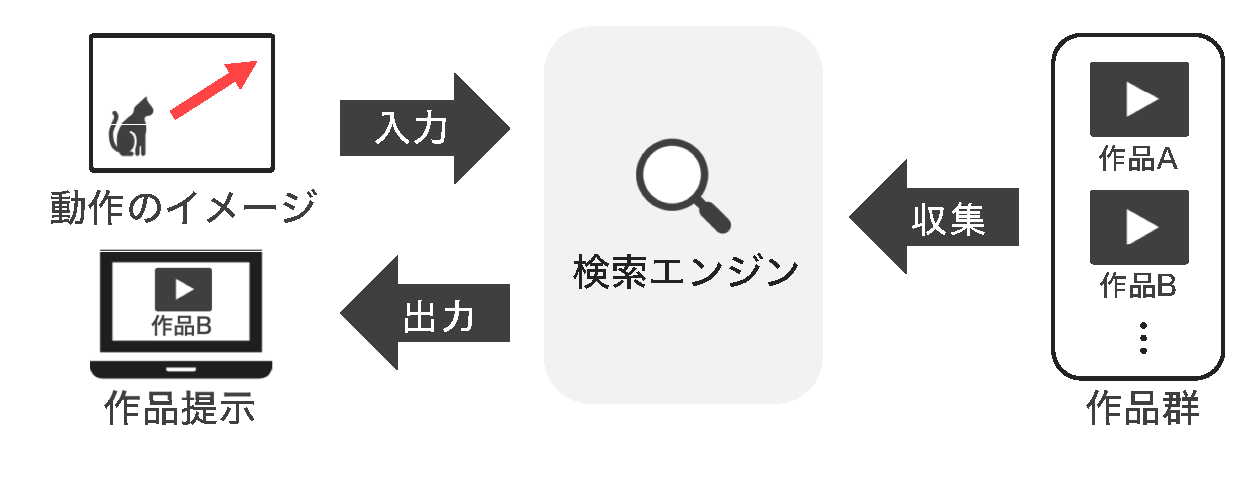
\includegraphics[width=15cm]{system.eps}
    \caption{Scratch作品の直感的検索システムの概略図}
    \label{searchsystem}
\end{figure}


\chapter{オブジェクトの動作に基づくScratch作品検索手法}

\section{概要}
本章では,動作のイメージを入力とするScratch作品の直感的検索手法を述べる.
図\ref{flow}は,手法の概略図を示す.
本論文では,\ref{scratchsetumei}節で説明したスクリプトによって画面上を動く
スプライトをオブジェクトと呼び,オブジェクトの動作を対象に検索を行う.
手順1では,入力となる動作のイメージの座標変化をマウス描画によって,
検索対象の作品に含まれるオブジェクトの動作の座標変化を画像認識によって取得する.
手順2では,入力と動作の類似性を測るために手順1で取得した座標変化同士の距離を算出する.
算出結果のうち,距離が近い動作を入力との類似動作として抽出する.

\begin{figure}[H]
    \centering
    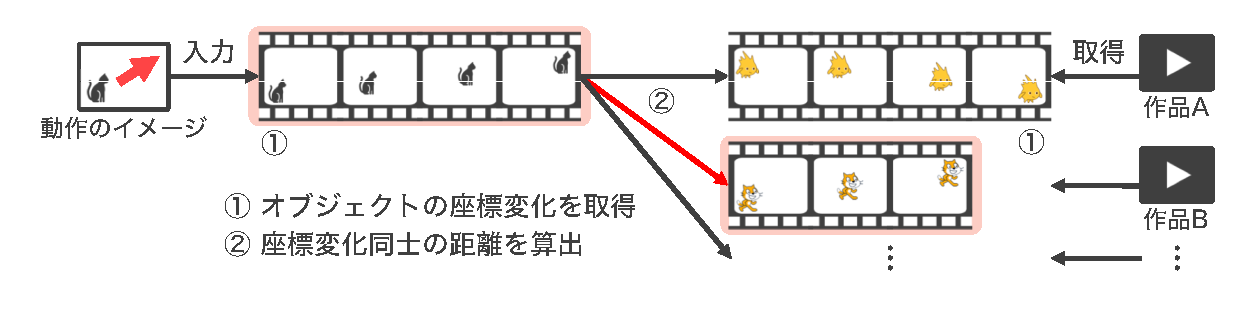
\includegraphics[width=15cm]{flow.eps}
    \caption{動作のイメージに基づく検索手法の概略図}
    \label{flow}
\end{figure}


\section{手順1: オブジェクトの座標変化を取得}
手順1では入力やオブジェクトの動作を捉えるために,
入力となる動作のイメージの座標変化をマウス描画によって,
検索対象の作品に含まれるオブジェクトの動作の座標変化を画像認識によって取得する.

\subsection{動作イメージの入力}
ユーザの持つ動作のイメージをマウスで描画することによって入力する.
動作のイメージを描画中,0.2秒ごとにマウスの座標を取得する.
取得した座標を,入力の座標変化の時系列データとする.

\subsection{検索対象作品に含まれるオブジェクトの動作}
\label{objectbehavior}

\subsubsection{検索対象作品の収集}
\label{collection}
Webアプリケーションの自動テストツールSelenium\footnote{https://www.selenium.dev/}を用いて,
Scratchのオンラインサービス上に公開されている作品のスナップショットを収集する.
スナップショットは,入力と同様の間隔で時系列データを取得するため0.2秒に1枚を収集する.
作品の中には実行が終わらない作品も存在するため,
該当する作品に対しては,最大100枚のスナップショットを収集する.
また,スナップショット収集を自動化するため,キー入力やマウス操作を必要としない作品を対象とする.

\subsubsection{画像認識による時系列データ取得}
収集した各作品のスナップショット中に存在するオブジェクトの座標変化を取得する.
座標変化の取得には,Loweが提案したSIFT(Scale-Invariant Feature Transform)\cite{sift}を用いた画像認識を行う.
SIFTは,画像中の特徴点検出と特徴量記述を行うアルゴリズムであり,照明変化や回転・拡大縮小に頑健である.
Scratchでは,オブジェクトとなるスプライトの色や回転・拡大縮小を自由に変更できるため,
そのような変更を含む作品にも画像認識が対応できるSIFTを採用する.
SIFTによる画像認識の手順は,以下の通りである.
\begin{enumerate}
     \item \textgt{スケール空間における極値検出:} 拡大縮小による不変性を得るため,対象とする点の特徴をより表現可能な
    近傍領域の範囲を決定する.近傍領域の範囲を決めるパラメータをスケールという.
    スケール$s$の異なるガウス関数$G(x,y,s)$と入力画像$I(x,y)$を畳み込んだ平滑化画像$L(x,y,s)$を
    式3.1,3.2により作成する.
    \begin{eqnarray}
        L(x,y,s) = G(x,y,s) * I(x,y) \\
        G(x,y,s) = \frac{1}{2\pi s^2} \exp (- \frac{x^2+y^2}{2s^2})
    \end{eqnarray}
    特徴点候補はスケールの異なる平滑化画像間の差分を取るDoG(Difference of Gaussian)画像$D(x,y,s)$から決定する.
    D(x,y,s)は式3.3から求める.
    \begin{eqnarray}
        D(x,y,s) = L(x,y,s_{i+1}) - L(x,y,s_i)
    \end{eqnarray}
    DoG画像を求める処理を複数の異なるスケール間で行うことで複数のDoG画像を取得し,
    得られたDoG画像から極値を検出する.
    極値の検出はDoG画像を3枚1組にして行う.
    極値を検出するDoG画像中のある画素に注目し,その周りの26近傍を比較する.
    注目画素が極値であった場合,その画素を特徴点候補として検出する.
    \item \textgt{特徴点のローカライズ:} 特徴点候補の中にはエッジ上の点が含まれており,ノイズの影響を受けやすい.
    そのため,エッジ上に存在する特徴点候補を削除することで安定した特徴点を絞り込む.
    エッジ上の特徴点候補を削除するために,各候補における二次元ヘッセ行列を式3.4から求める.
    \begin{eqnarray}
        H = \begin{bmatrix}
            D_{xx} & D_{xy} \\
            D_{xy} & D_{yy}
        \end{bmatrix}
    \end{eqnarray}
    Hから求められる第1固有値を$\alpha$,第2固有値を$\beta$とし,その比率を$\gamma$とすると式3.5が成り立つ.
    \begin{eqnarray}
        \alpha = \gamma\beta
    \end{eqnarray}
    よって,
    \begin{eqnarray}
        \frac{Tr(H)^2}{Det(H)} = \frac{(\alpha + \beta)^2}{\alpha\beta} = \frac{(\gamma + 1)^2}{\gamma}
    \end{eqnarray}
    となり,この値を閾値処理することで不要な特徴点の除去を行う.
    \item \textgt{回転角の計算:} 検出した各特徴点に対して,回転角を割り当てる.特徴点が検出された平滑化画像の
    各画素の勾配$m(x,y)$とその勾配方向$\theta(x,y)$を式3.7,3.8,3.9から求める.
    \begin{eqnarray}
        m(x,y) = \sqrt{f_x(x,y)^2 + f_y(x,y)^2} \\ 
        \theta(x,y) = \tan^{-1}\frac{f_y(x,y)}{f_x(x,y)}
    \end{eqnarray}
    \begin{eqnarray}
        \begin{cases}
            {f_x(x,y) = L(x+1,y) - L(x-1,y)} \\
            {f_y(x,y) = L(x,y+1) - L(x,y-1)} \\
        \end{cases}
    \end{eqnarray}
    求めた勾配$m$の大きさと勾配方向$\theta$から,重み付き方向ヒストグラムを作成する.
    作成したヒストグラムから最大値となる方向を特徴点の回転角として割り当てる.
    \item \textgt{特徴量の算出:} 特徴点の周辺領域を,手順3で割り当てた方向を基準とした軸に回転させる.
    軸を回転させた状態で特徴量を算出するため,回転に対する不変性を得ることができる.
    特徴点に対して周囲の$16×16$の画素を取り出し,この領域を16個の$4×4$の小領域の画素に分割する.
    各小領域に対してビンの数が8となるヒストグラムを作成する.
    結果として$8×16=128$個の特徴量が算出される.
    \item \textgt{特徴点のマッチング: } 2枚の画像間の特徴点のマッチングを,
    最も距離の近い点を探す最近傍探索によって行う.
\end{enumerate}

以上の手順で,スナップショット内に存在するオブジェクトの位置を特定する.
検出されたオブジェクトの中心座標を,座標変化の時系列データとする.
図\ref{recognition}は,スナップショット内に存在するオブジェクトを特定し,
そのオブジェクトの中心座標を取得した例を示す.
図\ref{recognition}の(1)はテンプレート画像を示し,(2)はスナップショットを示す.
テンプレート画像とスナップショットの間でマッチングした特徴点が,緑色の線で結ばれている.
青色の枠内にオブジェクトが検出され,青色の丸で中心座標が示されている.

\begin{figure}[H]
    \centering
    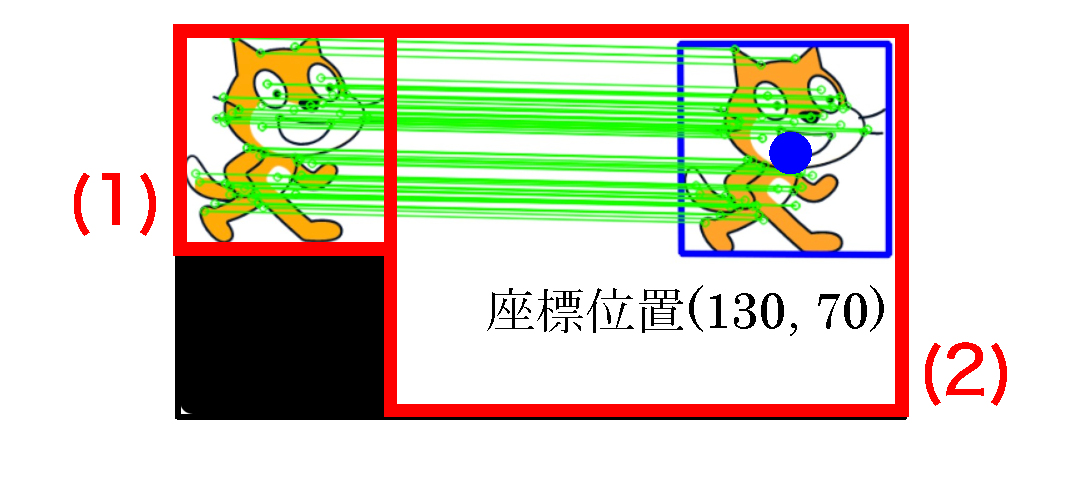
\includegraphics[width=7cm]{recognition.eps}
    \caption{画像認識の例}
    \label{recognition}
\end{figure}

本研究では,インテルが開発・公開しているオープンソースライブラリのOpenCV\footnote{https://opencv.org/}
を利用し,SIFTを用いた画像認識を行う.

Scratchでは,ユーザが自由にオブジェクトの画像を作成することができるため,
オンラインサービス上に公開されている作品で使用されているオブジェクト画像は多種多様である.
作品に含まれる全てのオブジェクトを対象に画像認識を行うことはできないため,
Scratchが標準画像として用意しているオブジェクト画像339件のみを画像認識のテンプレート画像とする.

本提案手法では,動作するオブジェクトを捉えるため,
オブジェクトの動作を命令する「動きブロック」を使用している作品を対象とする.
1作品には複数の動作を含んでいるため,連続したスナップショット中で
オブジェクトが登場しないフレームまでを1つの動作とする.


\section{手順2: 座標変化同士の距離を算出}

\subsection{時系列データの正規化}
本研究では,入力と検索対象動作の座標が離れている場合でも
軌跡が類似していれば類似動作として抽出する.
図\ref{moveexample}は,入力と検索対象動作の移動する座標が離れているが,軌跡が類似している例を示す.
図\ref{catmove}は入力を示し,画面中央を矢印の方向に移動している.
図\ref{dogmove}は検索対象動作を示し,画面下部を矢印の方向に移動している.
入力と検索対象動作が移動する座標は異なるが,いずれも矢印は右方向を向いているため,
類似動作として抽出する.
このような動作の抽出に対応するために,
手順1で取得した時系列データを最小値0,最大値1に正規化する.

\begin{figure}[H]
    \centering
    \begin{minipage}{0.45\linewidth}
        \centering
        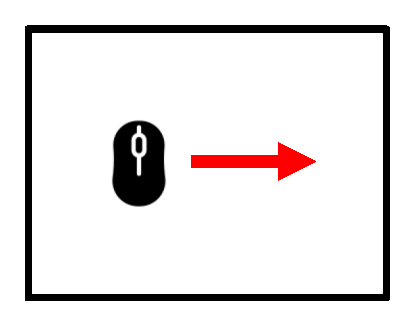
\includegraphics[height=3cm]{catmove.eps}
        \subcaption{入力の移動}
        \label{catmove}
    \end{minipage}
    \hspace{0.04\columnwidth}
    \begin{minipage}{0.45\linewidth}
        \centering
        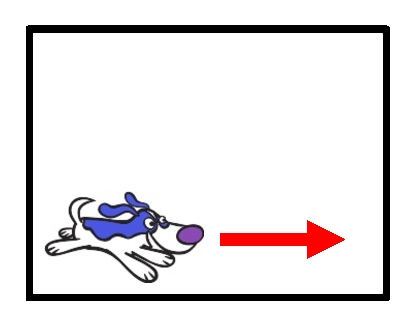
\includegraphics[height=3cm]{dogmove.eps}
        \subcaption{検索対象動作の移動}
        \label{dogmove}
    \end{minipage}
    \hspace{0.04\columnwidth}
    \caption{入力と検索対象動作の移動の例}
    \label{moveexample}
\end{figure}

\subsection{DTW距離の算出}
入力の座標変化と,検索対象動作の座標変化の距離を,
動的時間伸縮法(DTW: Dynamic time warping)を用いて算出する.
DTWは,2つの時系列データの距離を動的計画法に基づいて算出する手法である.
DTWでは2つの時系列データの各点の距離を総当たりで算出し,
全て求めた上で2つの時系列データの累積距離が最短となる経路を探し,
最短経路における累積距離が2つの時系列データの距離を示す.
異なる長さの時系列データ同士でも距離を算出可能である.
図\ref{dtw}に示すように,距離を算出する2つの時系列データ$S=s1,s2,...s15,T=t1,t2,...,t10$
を横軸と縦軸に並べ,各マス(i,j)における要素siとtj間の距離を算出する.
図中では,要素のマスの色が薄いほど距離が近く,濃いほど距離が遠いことを示す.
時系列データSとTの各要素の累積距離が最も短くなる経路を探すことで,2つの時系列データの距離を算出する.

\begin{figure}[H]
    \centering
    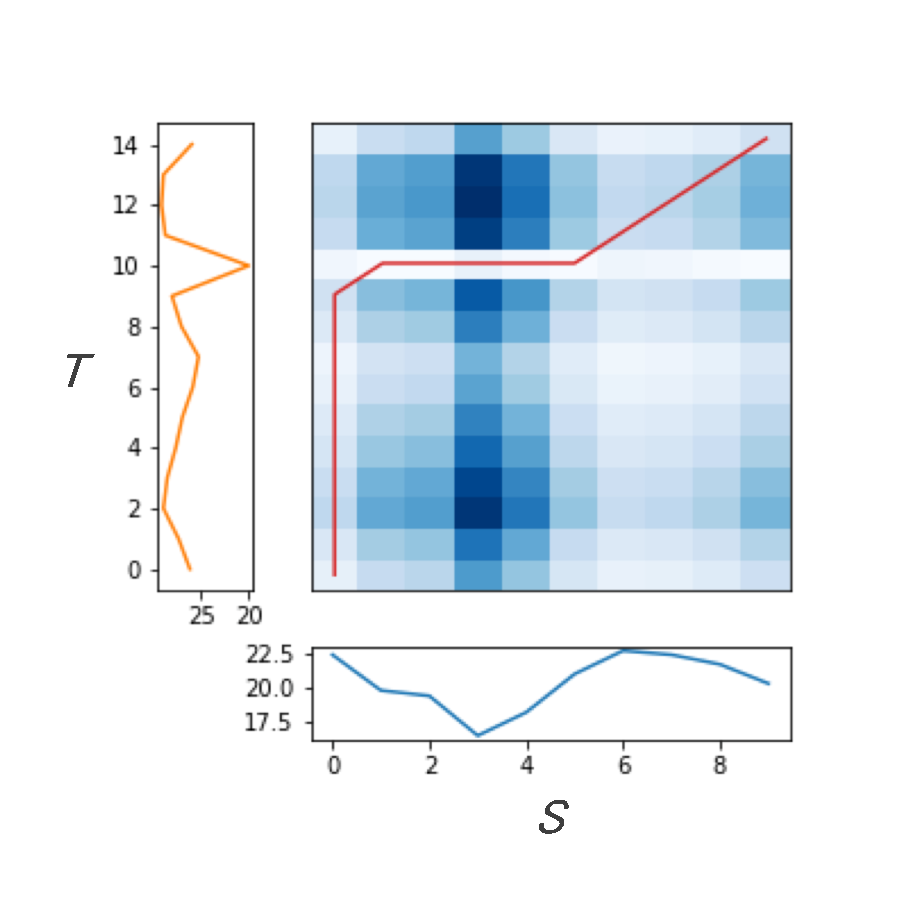
\includegraphics[height=10cm]{dtw.eps}
    \caption{動的時間伸縮法(DTW: Dynamic time warping)の概念図}
    \label{dtw}
\end{figure}

入力と検索対象動作の距離を求め,距離が近い動作を入力に類似する動作として抽出する.
距離は0に近いほど2つの時系列データが類似することを示し,値が大きくなるほど類似しないことを示す.

続く4章では,類似動作を抽出する距離と提案手法の検索精度について明らかにする.


\chapter{入力との距離算出結果の分析}
\label{analysys}

\section{概要}
本章では,入力に類似する動作を抽出可能な距離や提案手法の検索精度を明らかにするために,
著者が実装したScratch作品検索システムを用いて複数の入力を行い,
DTW距離の算出結果について分析を行う.
定量分析では,距離を昇順に並べたある2点の傾きから距離が収束する値を求めることで,
類似しない動作が抽出されるおおよその距離を明らかにする.
定性分析では,定量分析で明らかにした距離以下の動作を提示し,
動作の類似性を評価するアンケートを実施することで,類似動作を抽出可能な距離を明らかにする.
最後に,ランキング指標を用いた検索評価を行うことで,提案手法の検索精度を明らかにする.

\section{検索データセット}
Aivaloglouらの公開データセット\cite{dataset}\footnote{https://github.com/TUDelftScratchLab/ScratchDataset}
に含まれる作品233,491件の中から,次に示す条件を満たす13,437件の作品を用いる.
\begin{itemize}
    \item 表\ref{interactionblock}に示すユーザの操作を必要とするブロックを使用しない作品
    \item 動きブロックを使用した作品
    \item Scratchが標準画像として用意する画像を使用した作品
\end{itemize}

\begin{table}
    \caption{ユーザの操作を必要とするブロック}
    \label{interactionblock}
    \centering
    \begin{tabularx}{\textwidth}{l|l|X}
    \hline
        種類 & ブロック & 説明 \\
        \hline \hline
        \multirow{2}{*}{動きブロック} 
        & マウスポインターへ向ける & オブジェクトの向きをマウスポインターの方向に変更する \\
        \cline{2-3}
        & マウスポインターへ行く & オブジェクトをマウスポインターの位置に動かす \\
        \hline
        \multirow{2}{*}{イベントブロック}
        & (引数)キーが押されたとき & 引数に指定したキーが押された際にスクリプトを実行する \\
        \cline{2-3}
        & このスプライトが押されたとき & オブジェクトがクリックされた際にスクリプトを実行する \\
        \hline
        \multirow{7}{*}{調べるブロック} & マウスポインターに触れた & マウスポインターに触れたことを判定する \\
        \cline{2-3}
        & マウスポインターまでの距離 & オブジェクトとマウスポインター間のユークリッド距離を返す \\
        \cline{2-3}
        & (引数)と聞いて待つ & 引数に指定した文章と共に,画面下部にテキストの入力ボックスを表示する \\
        \cline{2-3}
        & (引数)キーが押された & 指定したキーが押されたことを判定する \\
        \cline{2-3}
        & マウスが押された & マウスが押されたことを判定する \\
        \cline{2-3}
        & マウスのx座標 & 現在のマウスポインターのx座標を返す \\
        \cline{2-3}
        & マウスのy座標 & 現在のマウスポインターのy座標を返す \\
        \hline
    \end{tabularx}
\end{table}

\section{検索システム}
本分析で入力・距離算出を行うために,著者が実装したScratch作品検索システムを用いる.
図\ref{systemdisplay}は検索画面を示す.
図\ref{systemdisplay}の(1)に示すキャンバスにマウス操作で動作のイメージの軌跡を入力し,
検索ボタンをクリックすることで入力と検索対象動作の距離算出を開始する.
全ての動作に対しての距離算出完了後,図\ref{systemdisplay}の(2)に示すように,
「各動作の含まれる作品のURL」「動作を行うスプライトの名称」「入力との距離」を,
距離の昇順に一覧表示する.

\begin{figure}[H]
    \centering
    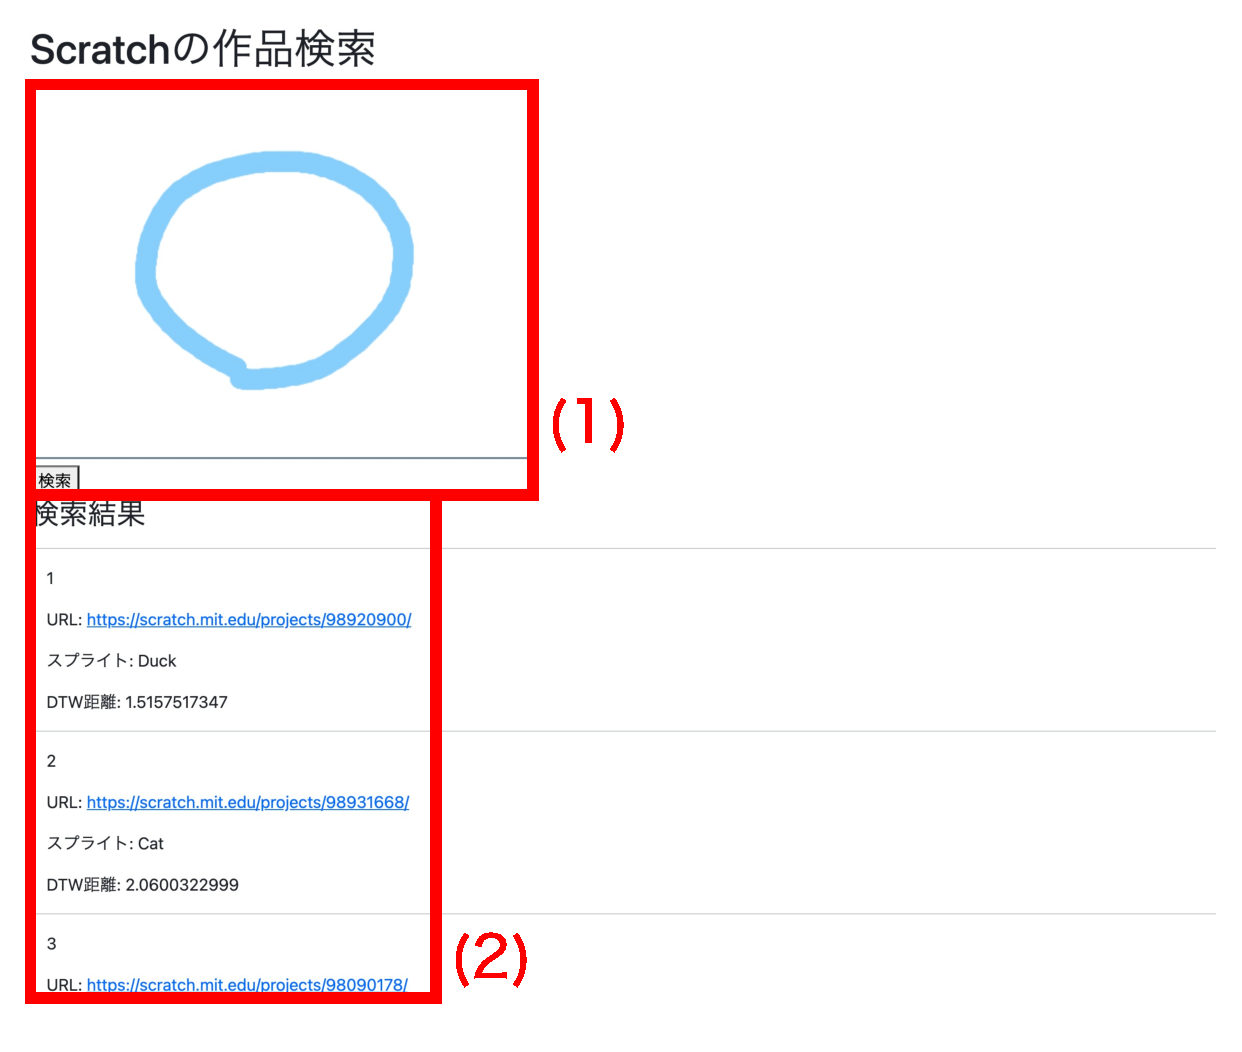
\includegraphics[height=8cm]{systemdisplay.eps}
    \caption{Scratch作品検索システムの画面}
    \label{systemdisplay}
\end{figure}

\section{入力}
オブジェクトの動作には,直線や曲線の移動があるため,直線・曲線移動を行う2つの動作を入力する.

\begin{itemize}
    \item 入力a: 左から右へ直線移動(図\ref{input1})
    \item 入力b: 左から上方向へ半円を描く曲線移動(図\ref{input2})
\end{itemize}

以上に加え,より長い動作を入力した場合の距離や動作の類似性についても確認するため,さらに2つの動作を入力する.

\begin{itemize}
    \item 入力c: 左上から時計回りに直線移動(図\ref{input3})
    \item 入力d: 左上から時計回りに曲線移動(図\ref{input4})
\end{itemize}

\begin{figure}[H]
    \centering
    \begin{minipage}{0.2\linewidth}
        \centering
        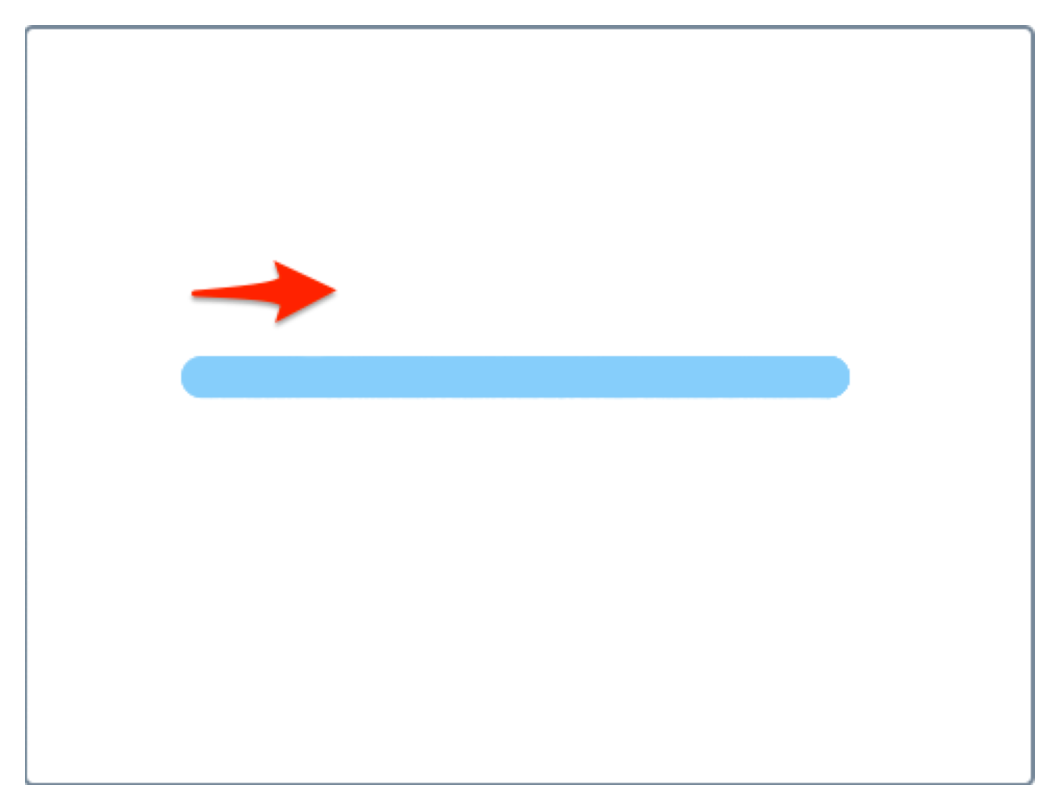
\includegraphics[height=2.5cm]{input1.eps}
        \subcaption{入力a}
        \label{input1}
    \end{minipage}
    \hspace{0.04\columnwidth}
    \begin{minipage}{0.2\linewidth}
        \centering
        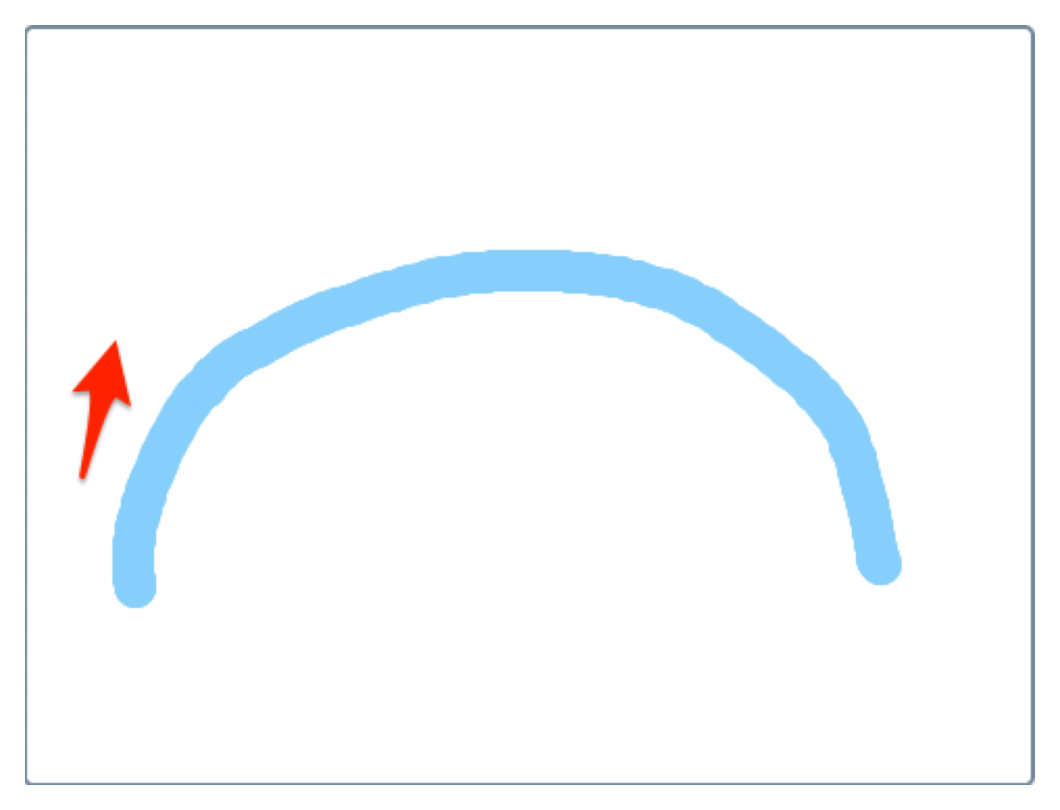
\includegraphics[height=2.5cm]{input2.eps}
        \subcaption{入力b}
        \label{input2}
    \end{minipage}
    \hspace{0.04\columnwidth}
    \begin{minipage}{0.2\linewidth}
        \centering
        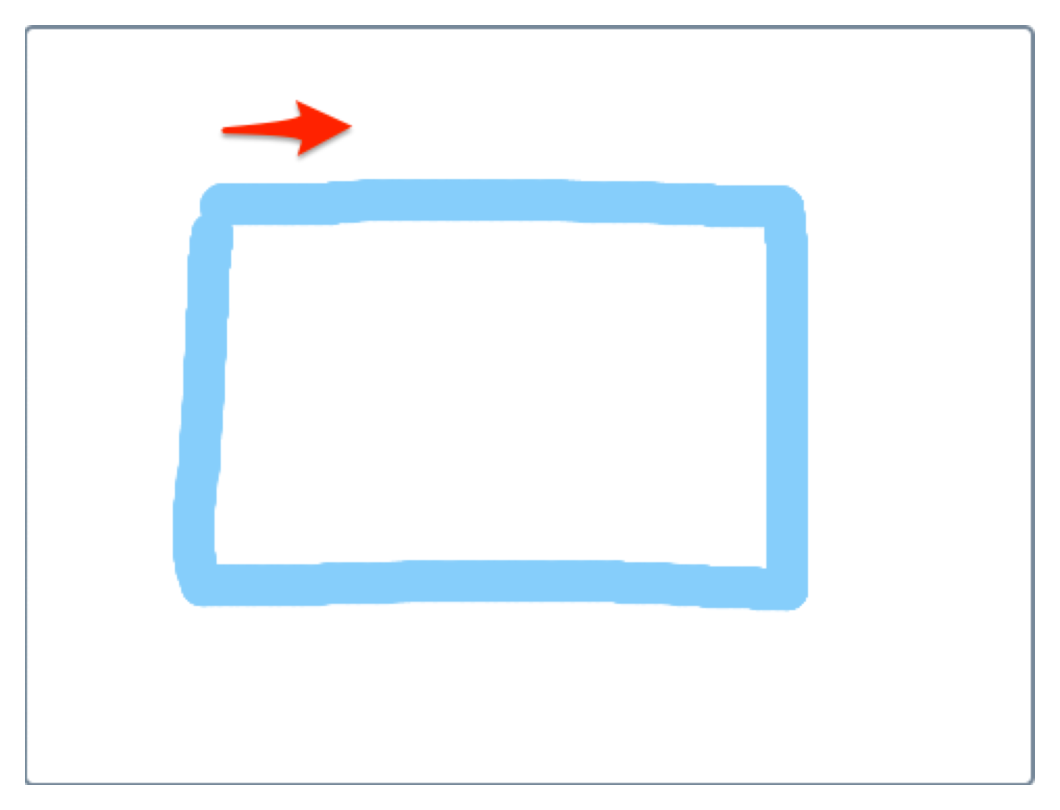
\includegraphics[height=2.5cm]{input3.eps}
        \subcaption{入力c}
        \label{input3}
    \end{minipage}
    \hspace{0.04\columnwidth}
    \begin{minipage}{0.2\linewidth}
        \centering
        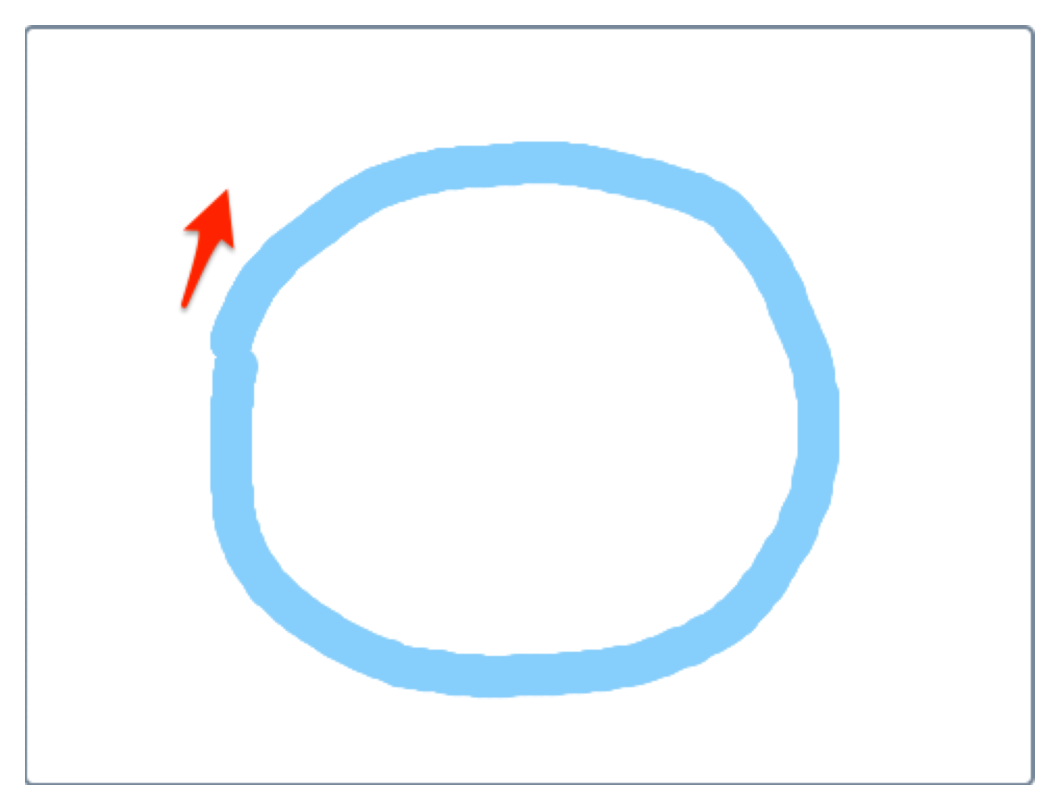
\includegraphics[height=2.5cm]{input4.eps}
        \subcaption{入力d}
        \label{input4}
    \end{minipage}
    \caption{分析で用いる4つの入力}
    \label{analyticsinput}
\end{figure}

\section{定量分析}
\label{teiryou}
定量分析では,類似しない動作を抽出するおおよその距離を明らかにするために,
距離を昇順に並べたある2点の傾きから収束する距離の値を,次に示す手順によって求める.

\begin{enumerate}
    \item 距離が近い動作から50件ごとに傾きを算出
    \item 傾きが0.5を切る距離の動作のスナップショットを目視で確認
    \item 2の結果,入力と類似しない動作であった場合,その距離を収束する距離とする
    \item 2の結果,入力と類似する動作であった場合,2以降の手順を再度行う
\end{enumerate}

各入力に対して定量分析を行なった結果を表\ref{quantitativeresult}に示す.
また,各入力の収束する値までの距離の散布図を図\ref{graph}に示す.

定量分析で明らかにした収束する距離は,
類似しない動作を抽出する距離として
\ref{teisei}の定性分析で実施するアンケートに提示する動作の抽出に用いる.
        
\begin{table}[H]
    \caption{移動方向が異なる動作が抽出される距離}
    \label{quantitativeresult}
    \centering
    \begin{tabular}{c|c}
    \hline
    入力 & 距離 \\
    \hline \hline
    a & 4.4 \\
    \hline
    b & 3.2 \\
    \hline
    c & 6.9 \\
    \hline
    d & 7.9 \\
    \hline
    \end{tabular}
\end{table}

\begin{figure}[htbp]
    \begin{tabular}{cc}
      \begin{minipage}[t]{0.45\hsize}
        \centering
        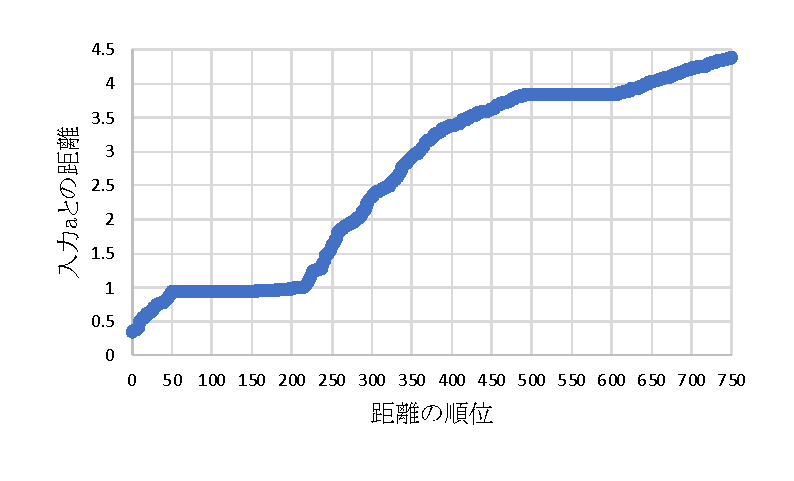
\includegraphics[height=4.5cm]{graph-a.eps}
        \subcaption{入力a}
        \label{graph-a}
      \end{minipage} &
      \hspace{0.04\columnwidth} 
      \begin{minipage}[t]{0.45\hsize}
        \centering
        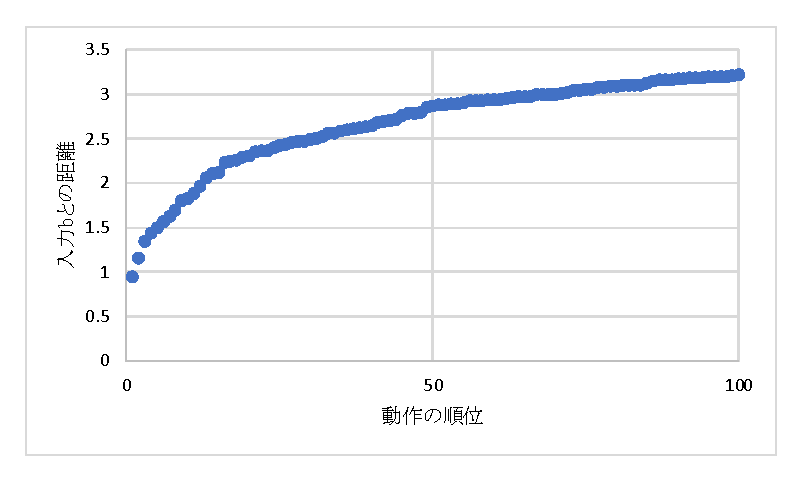
\includegraphics[height=4.5cm]{graph-b.eps}
        \subcaption{入力b}
        \label{graph-b}
      \end{minipage} \\
      \\
      \begin{minipage}[t]{0.45\hsize}
        \centering
        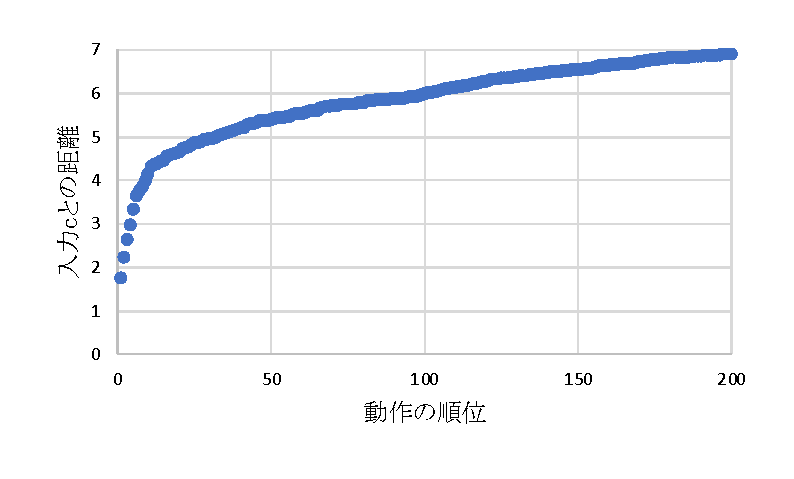
\includegraphics[height=4.5cm]{graph-c.eps}
        \subcaption{入力c}
        \label{graph-c}
      \end{minipage} &
      \hspace{0.04\columnwidth} 
      \begin{minipage}[t]{0.45\hsize}
        \centering
        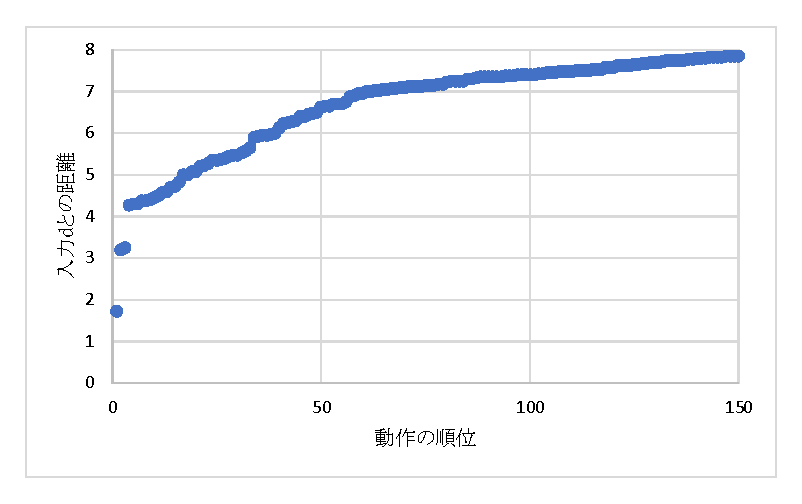
\includegraphics[height=4.5cm]{graph-d.eps}
        \subcaption{入力d}
        \label{graph-d}
      \end{minipage} 
    \end{tabular}
    \caption{入力と検索対象動作の距離の散布図}
    \label{graph}
\end{figure}


\section{定性分析}
\label{teisei}
定性分析では,入力に類似する動作を抽出可能な距離を明らかにするために,
入力と各検索対象動作のDTW距離算出結果から距離の異なる複数の動作を提示し,動作の類似性をアンケートで評価する.
アンケートに提示する動作は,\ref{teiryou}節で明らかにした類似しない動作を抽出する距離以下のものとする.
ただし,動作数が多いため,本分析では小数第2位を四捨五入した距離が重複するものは提示しない.
提示された動作が,入力と類似するかどうかを判断するために,次の1つ目の質問を設けた.

\begin{itemize}
    \item 質問1: スナップショットの動作は,入力に類似していますか?
\end{itemize}

質問1に対して,4段階のリッカート尺度(1: 類似する,2: やや類似する,3: やや類似しない,4: 類似しない)で評価を行う.
初めてアンケートの回答者全員が「4: 類似しない」を選択した距離を,類似動作を抽出可能な距離とする.
また,回答者にとってどのような理由で評価に繋がるかについて明らかにするために,
「1: 類似する」以外を選択した場合の理由を記述してもらった.

さらに,本研究は他者の作品を参照する学習の支援を期待するため,
提示された動作のプログラムを参考に,入力と類似する動作を実装できるかについて判断する2つ目の質問を設けた.

\begin{itemize}
    \item 質問2: プログラムを参考に入力と同じ動きを実装できますか?
\end{itemize}


質問2に対して,2値(1: 実装できる,2: 実装できない) で評価を行う.
アンケートの回答結果から,「動作は類似しており,プログラムも参考になる」
「動作は類似するがプログラムは参考にならない」といった事例の存在を明らかにする.

アンケートはプログラムの理解が必要であるため,Scratchのプログラムを理解できる著者を含む3名が回答した.

\subsubsection{入力a}
入力aのアンケート結果を表\ref{resulta}に示す.

\begin{itemize}
    \item 質問1: 最も距離の近い0.3(図\ref{a_0_3})から1.6(図\ref{a_1_6})の動作までは,
    回答者全員が「1: 類似する」を選択した.
    距離1.7(図\ref{a_1_7})の動作について1名の回答者が「2: やや類似する」を選択しており,
    選択理由を「移動距離が短いため」としている.
    距離3.2(図\ref{a_3_2})の動作では初めて「4: 類似しない」が選択された.
    1名の回答者が選択しており,選択理由を「移動距離が非常に短いため」としている.
    距離1.7と距離3.2の事例から,オブジェクトの移動方向が入力と類似する場合にも,
    回答者によっては移動距離を理由に類似しないと判断することが考えられる.
    距離4.3(図\ref{a_4_3})の動作では回答者全員が初めて「3: やや類似しない」を選択し,
    次の距離4.4(図\ref{a_4_4})の動作では回答者全員が初めて「4: 類似しない」を選択した.
    距離4.3の動作は,右方向へ移動しながらやや上方向への移動もしているため,
    回答者全員が「上方向への移動を含む」を理由に「3: やや類似しない」を選択した.
    また,距離4.4の動作は移動方向が類似していないために,回答者全員が「4: 類似しない」を選択した.
    距離4,3と距離4.4の事例から,移動方向が回答者全員の類似性の判断に影響することが考えられる.
    
    初めて回答者全員が「4: 類似しない」を選択した距離が4.3であるため,
    入力aとの類似動作を抽出可能な距離は4.3未満となる.
    
    \item 質問2: 最も距離の近い0.3から0.8(図\ref{a_0_8})の動作までは,回答者全員が「1: 実装できる」を選択した.
    距離0.9(図\ref{a_0_9})の動作について1名の回答者が「2: 実装できない」を選択した.
    距離0.9の動作のプログラムは,
    オブジェクトの持つ現在の「向き」に移動させる「(引数)歩動かす」ブロックを用いている.
    「2: 実装できない」を選択した回答者は自由記入欄に実装できない理由を記述しており,
    「オブジェクトの向きが左に初期化されているため,右方向への移動が実装できない」としている.
    一方,「1: 実装できる」を選択した回答者は「オブジェクトの向きを右に初期化することで実装できる」と述べている.
    距離0.9の事例から,オブジェクトの向きを入力の移動方向に初期化することで実装できる事例の存在が明らかになった.
    「2: 実装できない」が選択された他のいくつかの動作についても,移動方向の初期化により実装できる事例が見られた.
    距離4.4の動作は,質問1で回答者全員が「4: 類似しない」を選択したにもかかわらず,
    2名が「1: 実装できる」を選択した.
    距離4.4の動作は,距離0.9の動作と同様「(引数)歩動かす」ブロックを用いており,
    オブジェクトの向きを初期化することによって右方向への実装が可能となることから,
    動作は類似しないにもかかわらず,プログラムのみを見ることによって入力との類似動作を実装可能な事例の存在が
    明らかになった.
\end{itemize}

\subsubsection{入力b}
入力bのアンケート結果を表\ref{resultb}に示す.

\begin{itemize}
    \item 質問1: 最も距離の近い0.9(図\ref{b_0_9})と,
    2番目に距離の近い1.2(図\ref{b_1_2})の動作に対して,回答者全員が「1: 類似する」を選択した.
    距離1.5(図\ref{b_1_5})から1.8(図\ref{b_1_8})の動作まで1名の
    同じ回答者が「2: やや類似する」を選択している.
    いずれの動作も,入力より横方向の移動距離が短く縦方向の移動距離が長くなっていることから,
    選択理由として「角度が異なる」と述べている.
    また,距離1.6(図\ref{b_1_6})の動作について初めて「4: 類似しない」が選択された.
    1名の回答者が選択しており,理由として「(画面端に当たって)反射しているように見える」と述べている.
    距離1.5から1.8の動作の事例から,類似性の判断のために移動角度に着目することが考えられる.
    距離2.2(図\ref{b_2_2})の動作は左上から右下へ移動する動作であり,移動方向が類似しないために
    初めて回答者全員が「4: 類似しない」を選択した.
    以降の距離で,2つの動作で「移動方向は類似するが,曲線移動をしていない」などを理由に
    「2: やや類似する」が選択されたが,多くの動作で「3: やや類似しない」「4: 類似しない」が選択されている.
    距離2.8(図\ref{b_2_8})以降の全ての動作について,回答者全員が「4: 類似しない」を選択した.
    
    初めて回答者全員が「4: 類似しない」を選択した距離が2.2であるため,
    入力bとの類似動作を抽出可能な距離は2.2未満となる.
    
    \item 質問2: 最も距離の近い0.9から1.3(図\ref{b_1_3})の動作まで,回答者全員が「1: 実装できる」を選択した.
    距離1.4(図\ref{b_1_4})の動作について,質問1で「1: 類似する」「2: やや類似する」を選択したにもかかわらず,
    回答者全員が「2: 実装できない」を選択した.
    一見,入力のような曲線を描くように見えたが,プログラムは曲線移動でなく直線移動が実装されていることが
    明らかになった.そのため,回答者全員が入力のような動作を実装できないとしている.
    また,距離1.5や1.8の動作のプログラムはいずれもオブジェクトの向きを
    乱数を生成する「(引数1)から(引数2)までの乱数」ブロックで決定しているため,
    2名の回答者が「2: 実装できない」を選択した事例がみられた.
    本研究では「(引数1)から(引数2)までの乱数」ブロックを用いた作品を除外していないため,
    \ref{collection}項で作品を収集した際の実行結果に依存する.
    距離1.4や1.5,1.8などの動作から,
    動作が類似するにもかかわらず,プログラムを見ることで実際には入力のような実装ができない事例の存在が
    明らかになった.
    距離2.4(図\ref{b_2_4})以降の全ての動作について,回答者全員が「4: 実装できない」を選択した.
\end{itemize}    
    
\subsubsection{入力c}
入力cのアンケート結果を表\ref{resultc}に示す.

\begin{itemize}
    \item 質問1: 最も距離の近い1.7(図\ref{c_1_7})の動作に対して,回答者全員が「2: やや類似する」を選択した.
    距離1.7の動作は,入力同様,始点が左上の時計回りに四角形を描いているが,4辺のうち3辺が斜めに描かれるため,
    綺麗な四角形でないとして「2: やや類似する」を選択した.
    また,距離2.6(図\ref{c_2_6})の動作でも同様の理由で「2: やや類似する」あるいは「3: やや類似しない」が選択された.
    距離3.7(図\ref{c_3_7})から4.0(図\ref{c_4_0})までの動作は,いずれも同じ作品に含まれ,
    四角形を描く最初の右方向への1辺が短い,あるいは欠けている動作である.
    最初の右方向への1辺を理由に,1名が全てに対して「3: やや類似しない」を選択した.
    一方,「1: 類似する」「2: やや類似する」を選択した回答者もいる.
    距離3.3(図\ref{c_3_3})と3.8(図\ref{c_3_8})で「2: やや類似する」を選択した回答者は,
    理由として「一部動きが欠けており,方向転換の際に
    曲線を描いているように見えるが,全体的に類似している」と述べている.
    距離4.1(図\ref{c_4_1})の動作について,初めて回答者全員が「4: 類似しない」を選択した.
    また,距離4.1から4.4(図\ref{c_4_4})までの全ての動作について,四角形ではなく円を描く動作であることを理由に
    回答者全員が「4: 類似しない」を選択した.
    しかし,以降の距離には,2名以上が「1: 類似する」「2: やや類似する」を選択した動作が複数存在する.
    距離4.5(図\ref{c_4_5}),4.9(図\ref{c_4_9}),5.5(図\ref{c_5_5}),5,6(図\ref{c_5_6})は
    いずれも四角形の4つの頂点にのみ移動する動作であり,
    辺を描いて少しずつ移動するものではないが,
    「2: やや類似する」を選択した回答者は「頂点を移動しているが四角形に見える」と述べている.
    
    初めて回答者全員が「4: 類似しない」を選択した距離が4.1であるため,
    入力cとの類似動作を抽出可能な距離は4.1未満となる.
    
    \item 質問2: 最も距離の近い1.7から4.0の動作のうち,
    距離2.6の動作を除いて回答者全員が「1: 実装できる」を選択した.
    距離2.6の動作のプログラムは画面端に跳ね返りながら移動を繰り返す実装であり,
    四角形に移動させるための実装ではない.
    そのため, 距離2.6の動作について回答者全員が「2: 実装できない」を選択した.
    質問1では「2: やや類似する」を選択した回答者が2名いるため,
    動作が類似していても,プログラムを見ることで入力のような移動をするための実装がされていない動作の
    存在が明らかとなった.
    また,質問1で距離2.6の動作が綺麗な四角形でないと述べられた理由は,
    入力のような移動をするための実装でなかったためであると考えられる.
\end{itemize}

\subsubsection{入力d}
入力dのアンケート結果を表\ref{resultd}に示す.

\begin{itemize}
    \item 質問1: 回答者全員が「1: 類似する」を選択した動作は最も距離の近い1.7(図\ref{d_1_7})の動作のみとなった.
    以降の距離では「3: やや類似しない」「4: 類似しない」を多く選択している.
    距離4.5(図\ref{d_4_5})の動作において,初めて回答者全員が「4: 類似しない」を選択した.
    距離4.5の動作は,四角形に移動する動作であり,
    「4: 類似しない」を選択した理由として回答者全員が「四角形を描く直線移動である」と述べている.
    ただし,距離4.5以降において,2名以上が「2: やや類似する」を選択した動作も存在する.
    一例として,距離5.1(図\ref{d_5_1})の動作は入力よりも非常に小さい円を描いており,
    2名の回答者は円が小さいことを理由に「2: やや類似する」を選択した.
    残りの1名は,その場でオブジェクトが回転しているように見えるとして「4: 類似しない」を選択した.
    距離5.4(図\ref{d_5_4}),6.2(図\ref{d_6_2}),6.4(図\ref{d_6_4})の動作も同様の理由で同じ回答者が同じ選択をした.
    この事例から,回答者によって動作の見方が異なることが明らかになった.
    
    初めて回答者全員が「4: 類似しない」を選択した距離が4.5であるため,
    入力dとの類似動作を抽出可能な距離は4.5未満となる.

    \item 質問2: 質問1において,回答者全員が「1: 類似する」を選択した距離1.7の動作以外にも,
    回答者全員が「1: 実装できる」を選択した動作が見られる.
    質問1の結果において挙げた距離5.1,5.4,6.2,6.4の動作は,
    回答者全員が「1: 実装できる」を選択した.
    自由記述欄にて,質問1で「4: 類似しない」を選択した回答者は
    「プログラムを見ることで,その場でオブジェクトが回転しているのではなく,円を描いていることがわかった」
    と述べている.
    一見動作が類似していなくても,プログラムを参照することにより実装可能な類似動作を
    発見できることが明らかになった.
\end{itemize}

\begin{table}[H]
    \caption{入力aのアンケート結果}
    \label{resulta}
    \centering
    \scalebox{0.8}{
    \begin{tabular}{c|c|c|c|c|c|c}
    \hline
     & \multicolumn{4}{c|}{質問1の回答数} & \multicolumn{2}{c}{質問2の回答数} \\
    \hline
    距離 & 1: 類似する & 2: やや類似する & 3: やや類似しない & 4: 類似しない & 1: 実装できる & 2: 実装できない \\
    \hline \hline
    0.3 & 3 & 0 & 0 & 0 & 3 & 0 \\
    \hline
    0.4 & 3 & 0 & 0 & 0 & 3 & 0 \\
    \hline
    0.5 & 3 & 0 & 0 & 0 & 3 & 0 \\
    \hline
    0.6 & 3 & 0 & 0 & 0 & 3 & 0 \\
    \hline
    0.7 & 3 & 0 & 0 & 0 & 3 & 0 \\
    \hline
    0.8 & 3 & 0 & 0 & 0 & 3 & 0 \\
    \hline
    0.9 & 3 & 0 & 0 & 0 & 2 & 1 \\
    \hline
    1.0 & 3 & 0 & 0 & 0 & 2 & 1 \\
    \hline
    1.1 & 3 & 0 & 0 & 0 & 3 & 0 \\
    \hline
    1.2 & 3 & 0 & 0 & 0 & 2 & 1 \\
    \hline
    1.3 & 3 & 0 & 0 & 0 & 3 & 0 \\
    \hline
    1.4 & 3 & 0 & 0 & 0 & 3 & 0 \\
    \hline
    1.5 & 3 & 0 & 0 & 0 & 3 & 0 \\
    \hline
    1.6 & 3 & 0 & 0 & 0 & 3 & 0 \\
    \hline
    1.7 & 2 & 1 & 0 & 0 & 3 & 0 \\
    \hline
    1.8 & 3 & 0 & 0 & 0 & 3 & 0 \\
    \hline
    1.9 & 3 & 0 & 0 & 0 & 3 & 0 \\
    \hline
    2.0 & 2 & 1 & 0 & 0 & 3 & 0 \\
    \hline
    2.1 & 2 & 1 & 0 & 0 & 3 & 0 \\
    \hline
    2.2 & 2 & 0 & 1 & 0 & 2 & 1 \\
    \hline
    2.3 & 3 & 0 & 0 & 0 & 3 & 0 \\
    \hline
    2.4 & 1 & 1 & 1 & 0 & 3 & 0 \\
    \hline
    2.5 & 3 & 0 & 0 & 0 & 3 & 0 \\
    \hline
    2.6 & 2 & 0 & 1 & 0 & 3 & 0 \\
    \hline
    2.7 & 3 & 0 & 0 & 0 & 3 & 0 \\
    \hline
    2.8 & 3 & 0 & 0 & 0 & 3 & 0 \\
    \hline
    2.9 & 3 & 0 & 0 & 0 & 3 & 0 \\
    \hline
    3.0 & 0 & 3 & 0 & 0 & 3 & 0 \\
    \hline
    3.1 & 3 & 0 & 0 & 0 & 3 & 0 \\
    \hline
    3.2& 2 & 0 & 0 & 1 & 1 & 2 \\
    \hline
    3.3 & 3 & 0 & 0 & 0 & 3 & 0 \\
    \hline
    3.4 & 1 & 0 & 2 & 0 & 3 & 0 \\
    \hline
    3.5 & 3 & 0 & 0 & 0 & 2 & 1 \\
    \hline
    3.6 & 3 & 0 & 0 & 0 & 3 & 0 \\
    \hline
    3.7 & 1 & 0 & 2 & 0 & 2 & 1 \\
    \hline
    3.8 & 3 & 0 & 0 & 0 & 3 & 0 \\
    \hline
    3.9 & 2 & 1 & 0 & 0 & 3 & 0 \\
    \hline
    4.0 & 0 & 1 & 2 & 0 & 3 & 0 \\
    \hline
    4.1 & 3 & 0 & 0 & 0 & 3 & 0 \\
    \hline
    4.2 & 3 & 0 & 0 & 0 & 3 & 0 \\
    \hline
    4.3 & 0 & 0 & 3 & 0 & 1 & 2 \\
    \hline
    4.4 & 0 & 0 & 0 & 3 & 2 & 1 \\
    \hline
    \end{tabular}
    }
\end{table}

\begin{figure}[H]
    \begin{tabular}{cc}
      \begin{minipage}[t]{0.45\hsize}
        \centering
        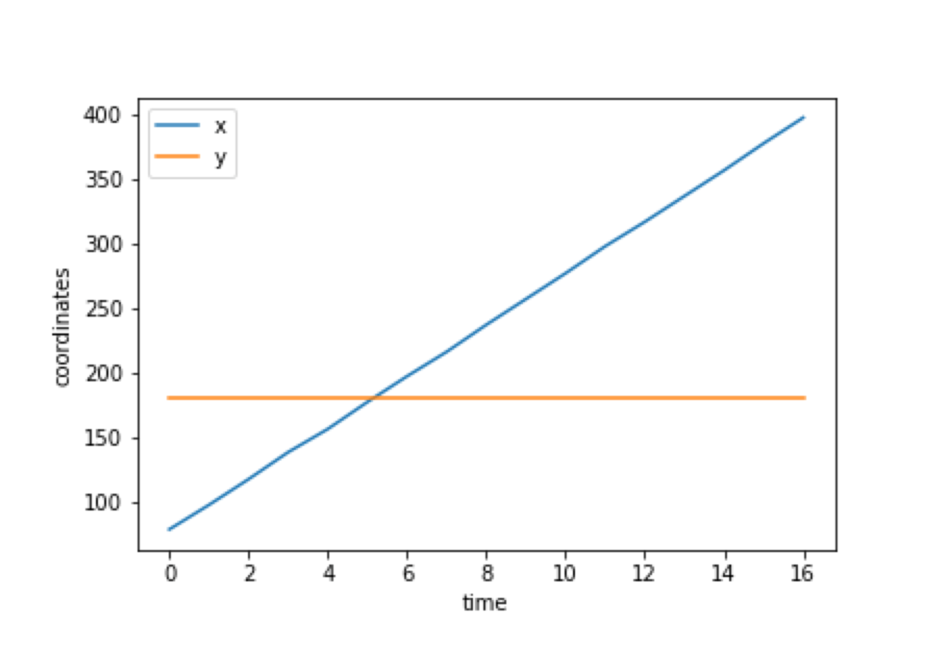
\includegraphics[height=5cm]{a_0_3.eps}
        \subcaption{距離0.3の動作の座標変化}
        \label{a_0_3}
      \end{minipage} &
      \begin{minipage}[t]{0.45\hsize}
        \centering
        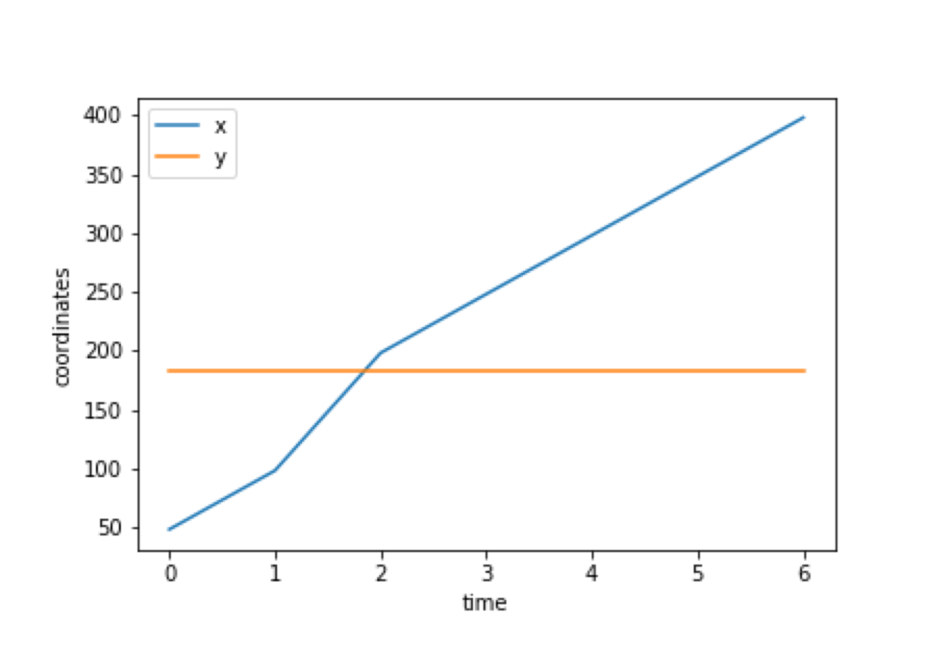
\includegraphics[height=5cm]{a_0_8.eps}
        \subcaption{距離0.8の動作の座標変化}
        \label{a_0_8}
      \end{minipage} \\
   
      \begin{minipage}[t]{0.45\hsize}
        \centering
        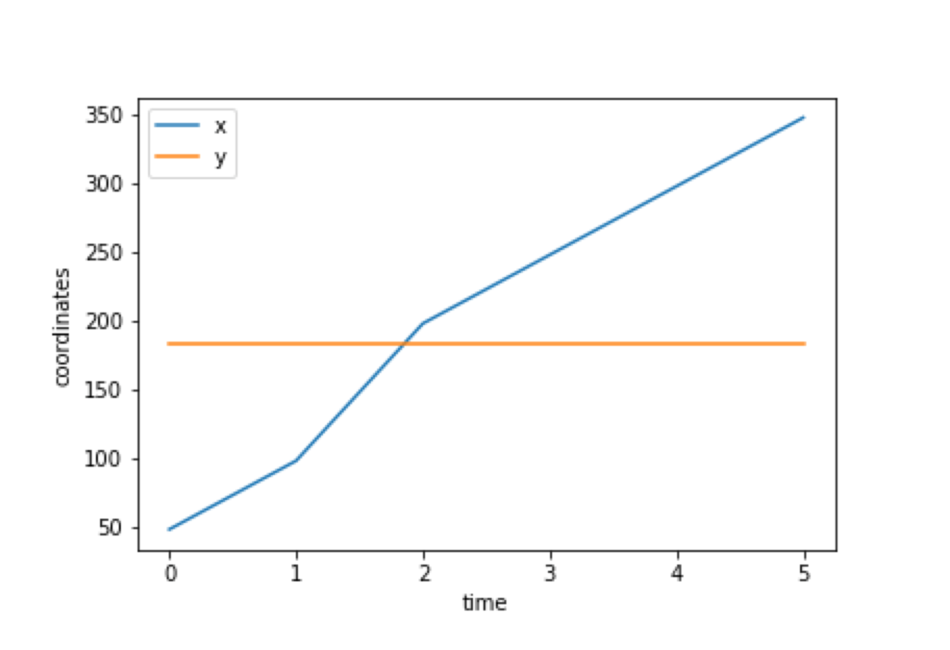
\includegraphics[height=5cm]{a_0_9.eps}
        \subcaption{距離0.9の動作の座標変化}
        \label{a_0_9}
      \end{minipage} &
      \begin{minipage}[t]{0.45\hsize}
        \centering
        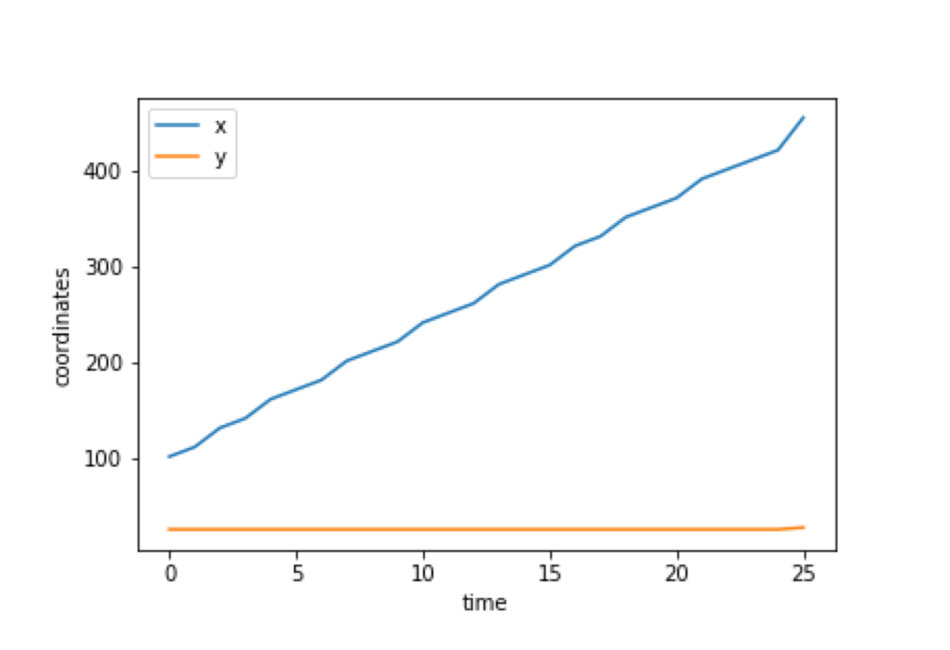
\includegraphics[height=5cm]{a_1_6.eps}
        \subcaption{距離1.6の動作の座標変化}
        \label{a_1_6}
      \end{minipage} \\
      
      \begin{minipage}[t]{0.45\hsize}
        \centering
        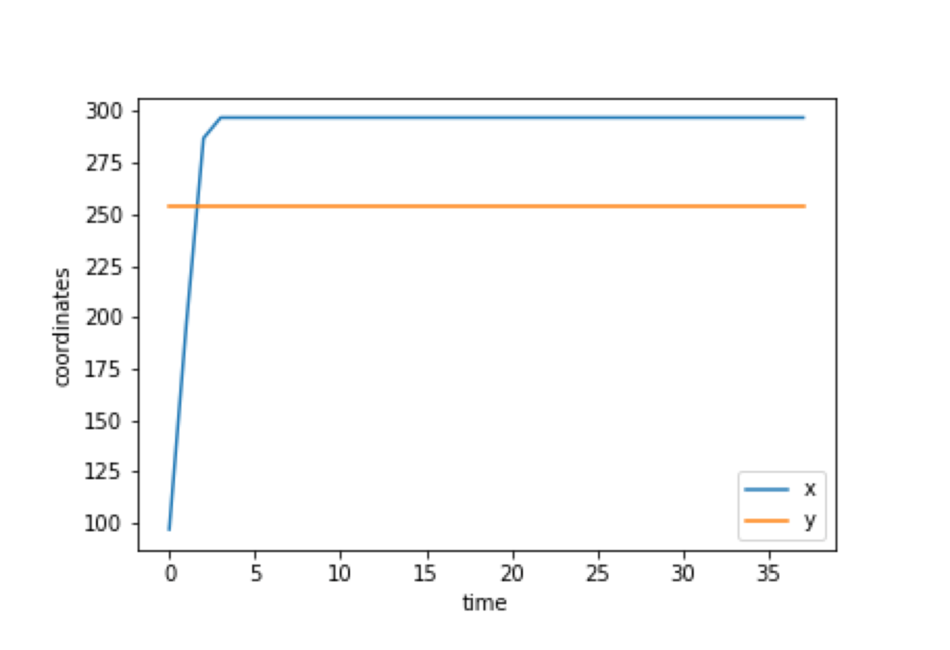
\includegraphics[height=5cm]{a_1_7.eps}
        \subcaption{距離1.7の動作の座標変化}
        \label{a_1_7}
      \end{minipage} &
      \begin{minipage}[t]{0.45\hsize}
        \centering
        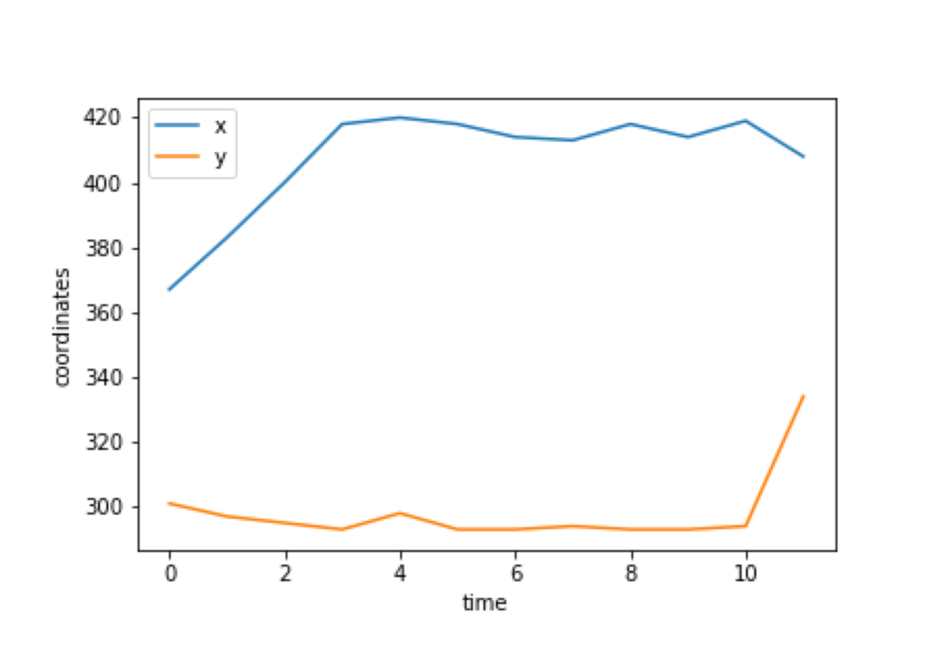
\includegraphics[height=5cm]{a_3_2.eps}
        \subcaption{距離3.2の動作の座標変化}
        \label{a_3_2}
      \end{minipage} \\
      
      \begin{minipage}[t]{0.45\hsize}
        \centering
        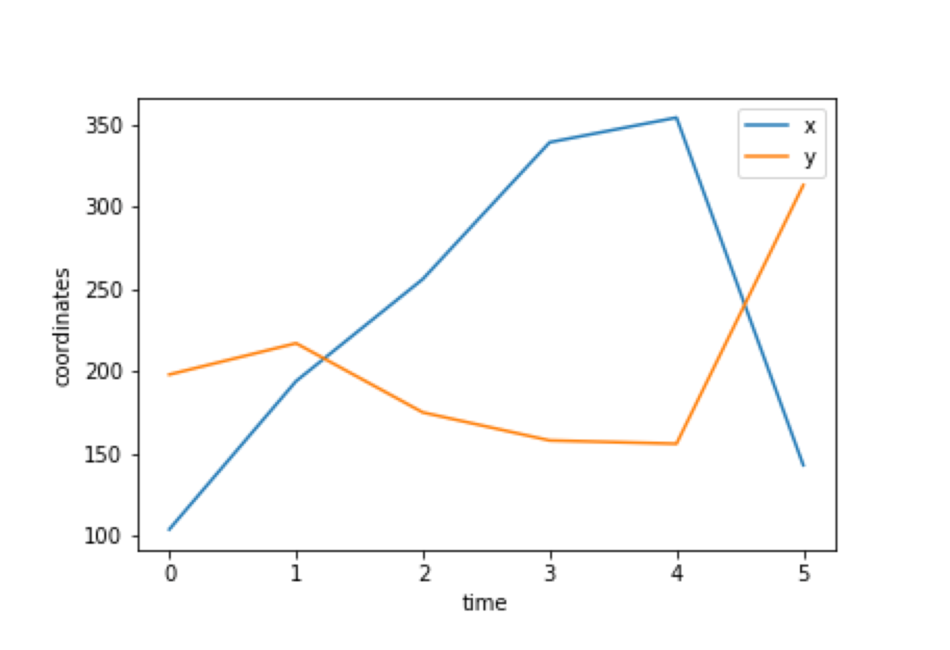
\includegraphics[height=5cm]{a_4_3.eps}
        \subcaption{距離4.3の動作の座標変化}
        \label{a_4_3}
      \end{minipage} &
      \begin{minipage}[t]{0.45\hsize}
        \centering
        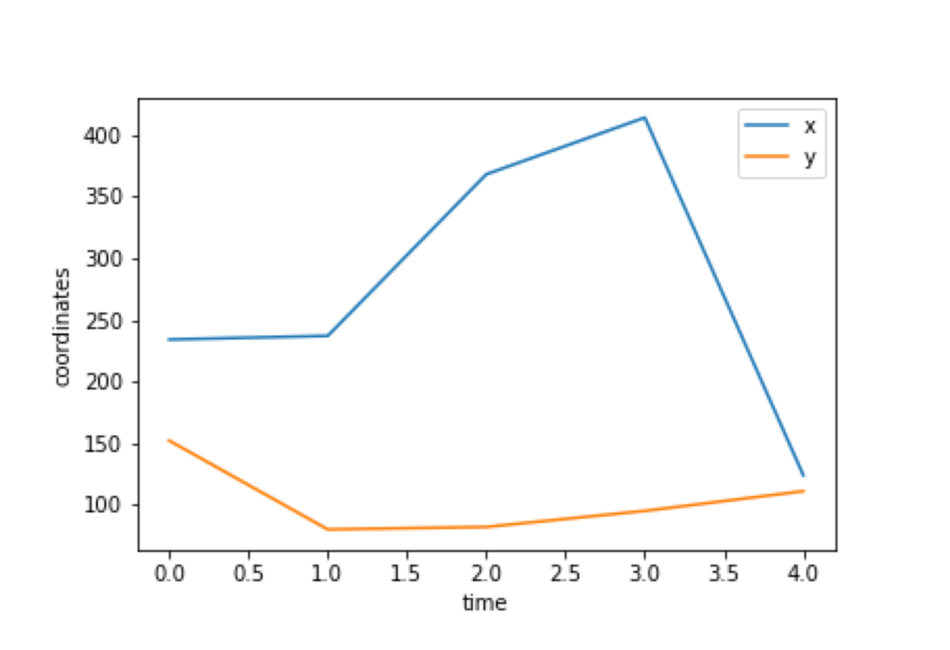
\includegraphics[height=5cm]{a_4_4.eps}
        \subcaption{距離4.4の動作の座標変化}
        \label{a_4_4}
      \end{minipage} \\
    \end{tabular}
    \caption{入力aのアンケートに提示した動作の例}
    \label{inputa-ex}
\end{figure}

\begin{table}[H]
    \caption{入力bのアンケート結果}
    \label{resultb}
    \centering
    \scalebox{0.8}{
    \begin{tabular}{c|c|c|c|c|c|c}
    \hline
     & \multicolumn{4}{c|}{質問1の回答数} & \multicolumn{2}{c}{質問2の回答数} \\
    \hline
    距離 & 1: 類似する & 2: やや類似する & 3: やや類似しない & 4: 類似しない & 1: 実装できる & 2: 実装できない \\
    \hline \hline
    0.9 & 3 & 0 & 0 & 0 & 3 & 0 \\
    \hline
    1.2 & 3 & 0 & 0 & 0 & 3 & 0 \\
    \hline
    1.3 & 2 & 1 & 0 & 0 & 2 & 1 \\
    \hline
    1.4 & 2 & 1 & 0 & 0 & 0 & 3 \\
    \hline
    1.5 & 2 & 1 & 0 & 0 & 1 & 2 \\
    \hline
    1.6 & 1 & 1 & 0 & 1 & 1 & 2 \\
    \hline
    1.7 & 1 & 2 & 0 & 0 & 1 & 2 \\
    \hline
    1.8 & 2 & 1 & 0 & 0 & 1 & 2 \\
    \hline
    1.9 & 1 & 1 & 0 & 1 & 1 & 2 \\
    \hline
    2.0 & 1 & 2 & 0 & 0 & 0 & 3 \\
    \hline
    2.1 & 2 & 0 & 1 & 0 & 2 & 1 \\
    \hline
    2.2 & 0 & 0 & 0 & 3 & 0 & 3 \\
    \hline
    2.3 & 0 & 2 & 0 & 1 & 1 & 2 \\
    \hline
    2.4 & 0 & 0 & 1 & 2 & 0 & 3 \\
    \hline
    2.5 & 0 & 1 & 2 & 0 & 0 & 3 \\
    \hline
    2.6 & 0 & 0 & 0 & 3 & 0 & 3 \\
    \hline
    2.7 & 0 & 0 & 3 & 0 & 0 & 3 \\
    \hline
    2,8 & 0 & 0 & 0 & 3 & 0 & 3 \\
    \hline
    2.9 & 0 & 0 & 0 & 3 & 0 & 3 \\
    \hline
    3.0 & 0 & 0 & 0 & 3 & 0 & 3 \\
    \hline
    3.1 & 0 & 0 & 0 & 3 & 0 & 3 \\
    \hline
    3.2 & 0 & 0 & 0 & 3 & 0 & 3 \\
    \hline
    \end{tabular}
    }
\end{table}

\begin{figure}[H]
    \begin{tabular}{cc}
      \begin{minipage}[t]{0.45\hsize}
        \centering
        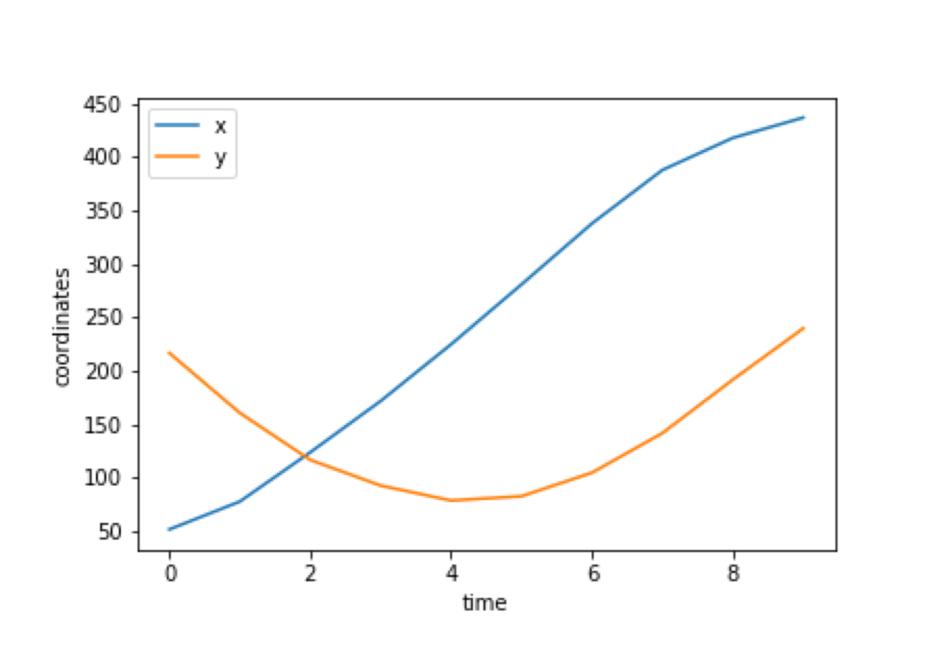
\includegraphics[height=5cm]{b_0_9.eps}
        \subcaption{距離0.9の動作の座標変化}
        \label{b_0_9}
      \end{minipage} &
      \begin{minipage}[t]{0.45\hsize}
        \centering
        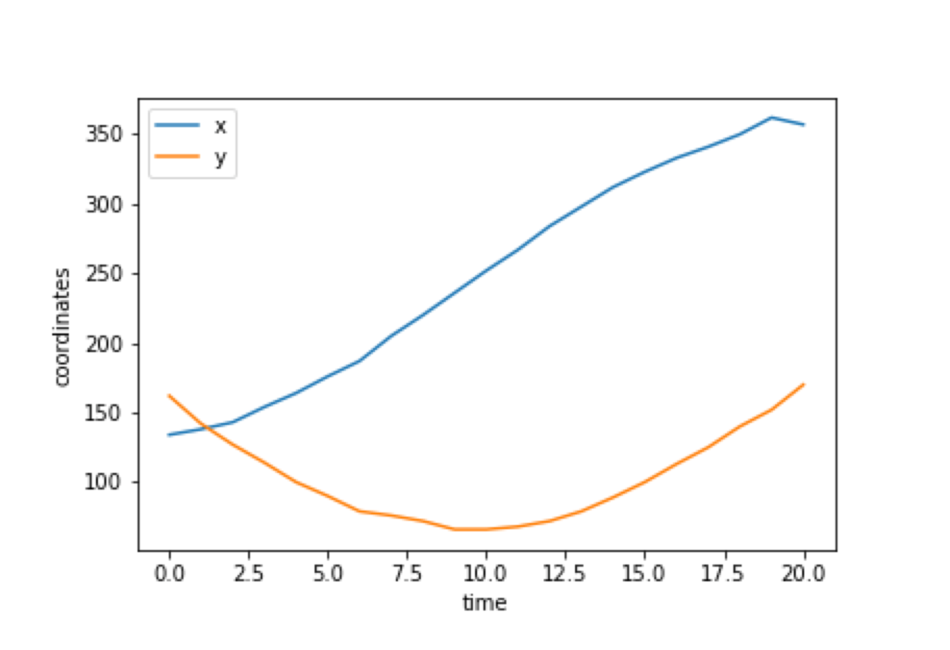
\includegraphics[height=5cm]{b_1_2.eps}
        \subcaption{距離1.2の動作の座標変化}
        \label{b_1_2}
      \end{minipage} \\
   
      \begin{minipage}[t]{0.45\hsize}
        \centering
        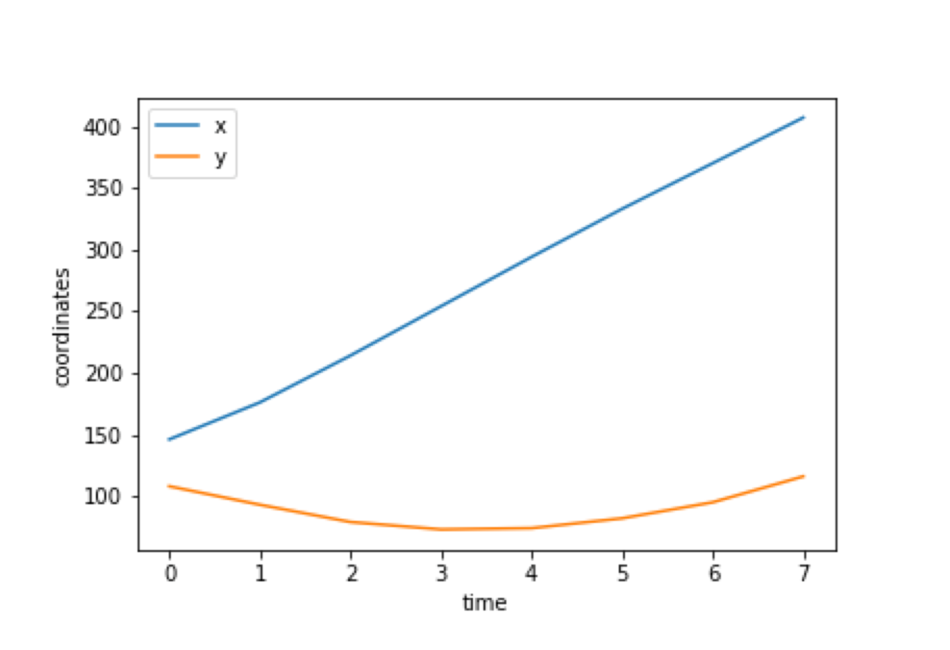
\includegraphics[height=5cm]{b_1_3.eps}
        \subcaption{距離1.3の動作の座標変化}
        \label{b_1_3}
      \end{minipage} &
      \begin{minipage}[t]{0.45\hsize}
        \centering
        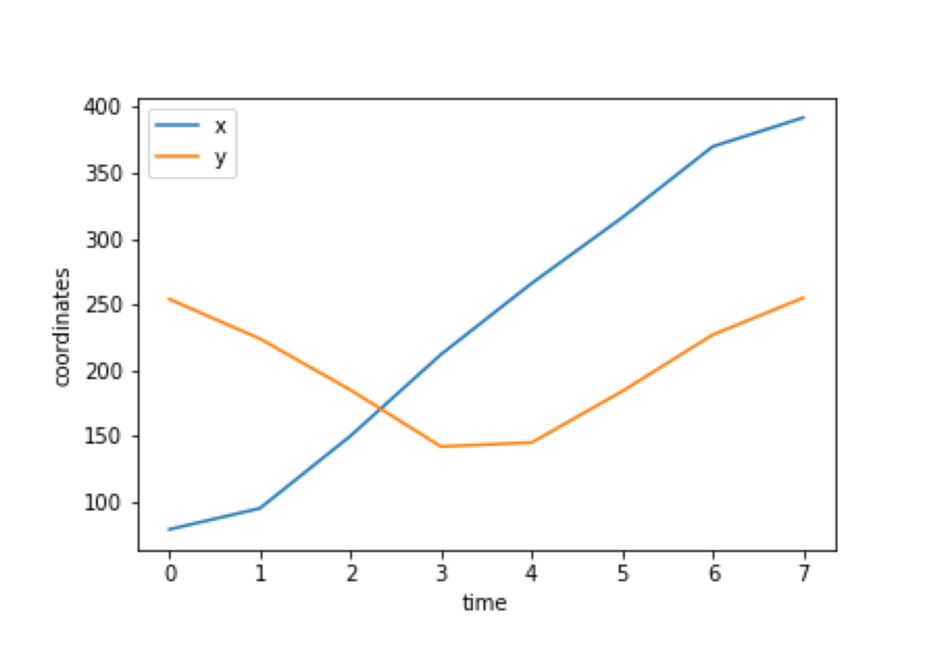
\includegraphics[height=5cm]{b_1_4.eps}
        \subcaption{距離1.4の動作の座標変化}
        \label{b_1_4}
      \end{minipage} \\
      
      \begin{minipage}[t]{0.45\hsize}
        \centering
        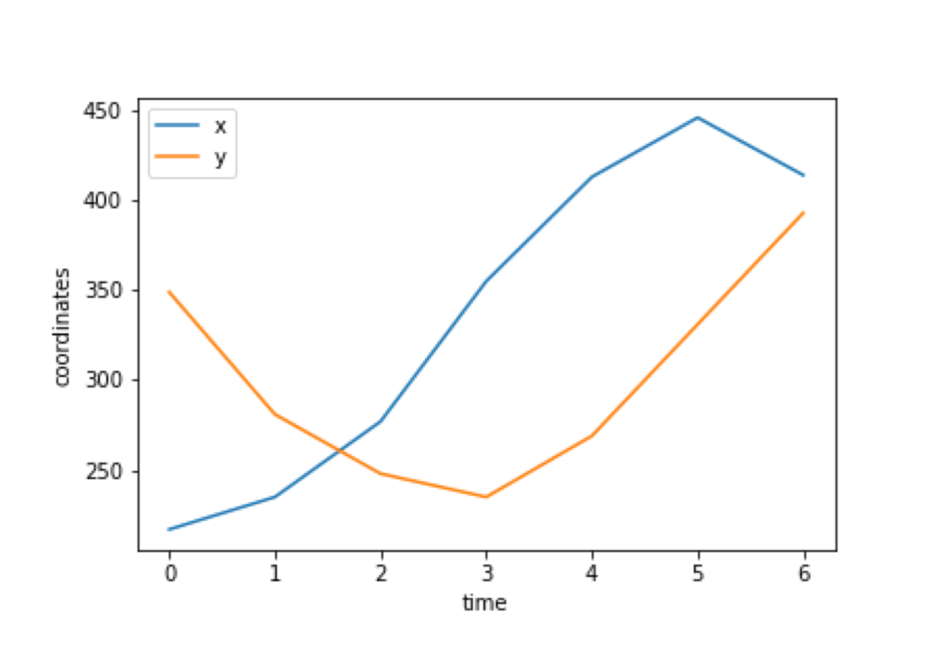
\includegraphics[height=5cm]{b_1_5.eps}
        \subcaption{距離1.5の動作の座標変化}
        \label{b_1_5}
      \end{minipage} &
      \begin{minipage}[t]{0.45\hsize}
        \centering
        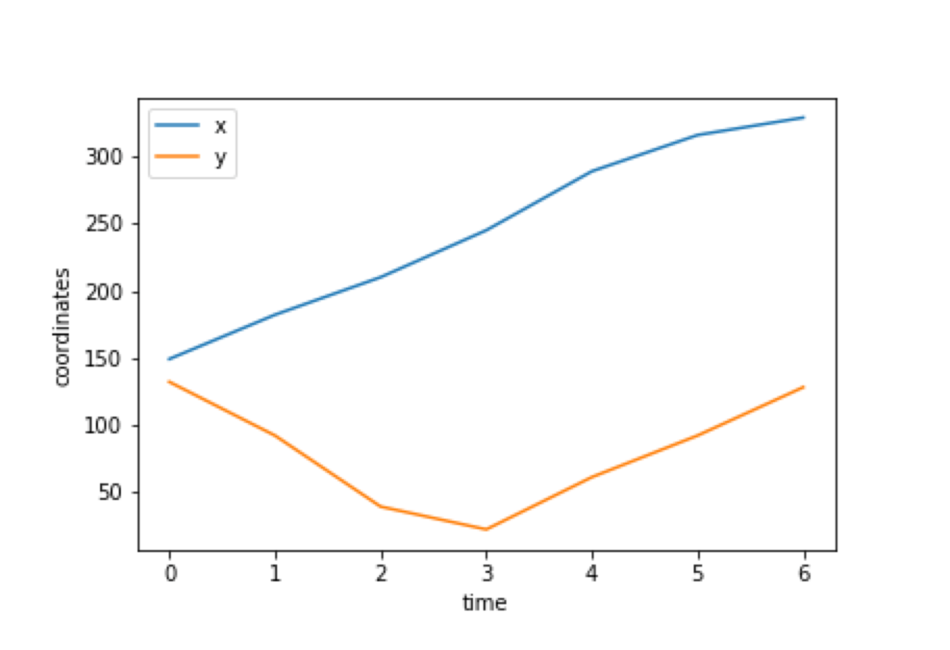
\includegraphics[height=5cm]{b_1_6.eps}
        \subcaption{距離1.6の動作の座標変化}
        \label{b_1_6}
      \end{minipage} \\
      
      \begin{minipage}[t]{0.45\hsize}
        \centering
        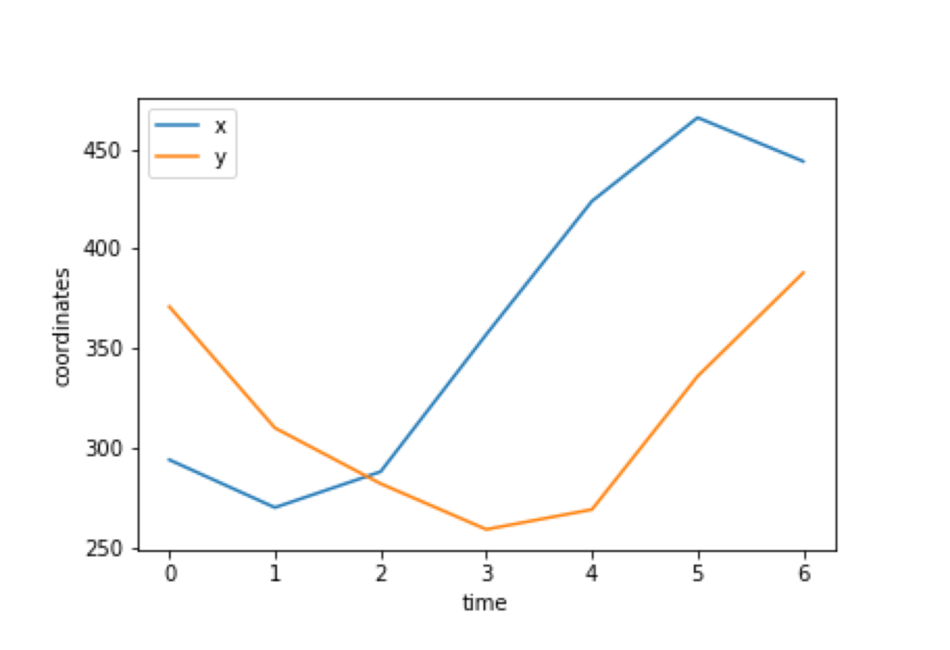
\includegraphics[height=5cm]{b_1_8.eps}
        \subcaption{距離1.8の動作の座標変化}
        \label{b_1_8}
      \end{minipage} &
      \begin{minipage}[t]{0.45\hsize}
        \centering
        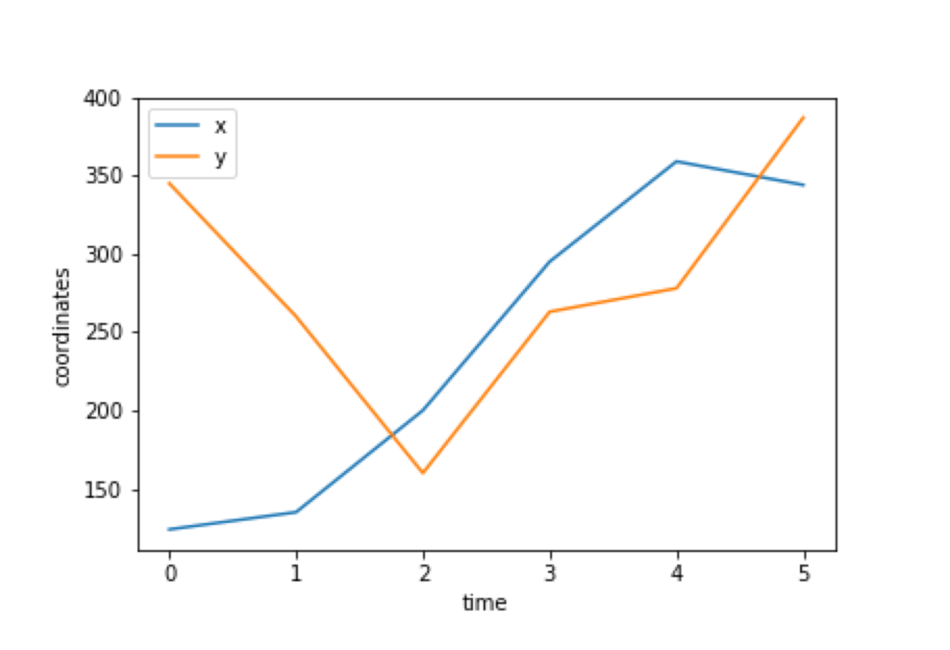
\includegraphics[height=5cm]{b_2_2.eps}
        \subcaption{距離2.2の動作の座標変化}
        \label{b_2_2}
      \end{minipage}
      \end{tabular}
    \caption{入力bのアンケートに提示した動作の例1}
    \label{inputb-ex}
\end{figure}

\begin{figure}[H]
    \begin{tabular}{cc}
      \begin{minipage}[t]{0.45\hsize}
        \centering
        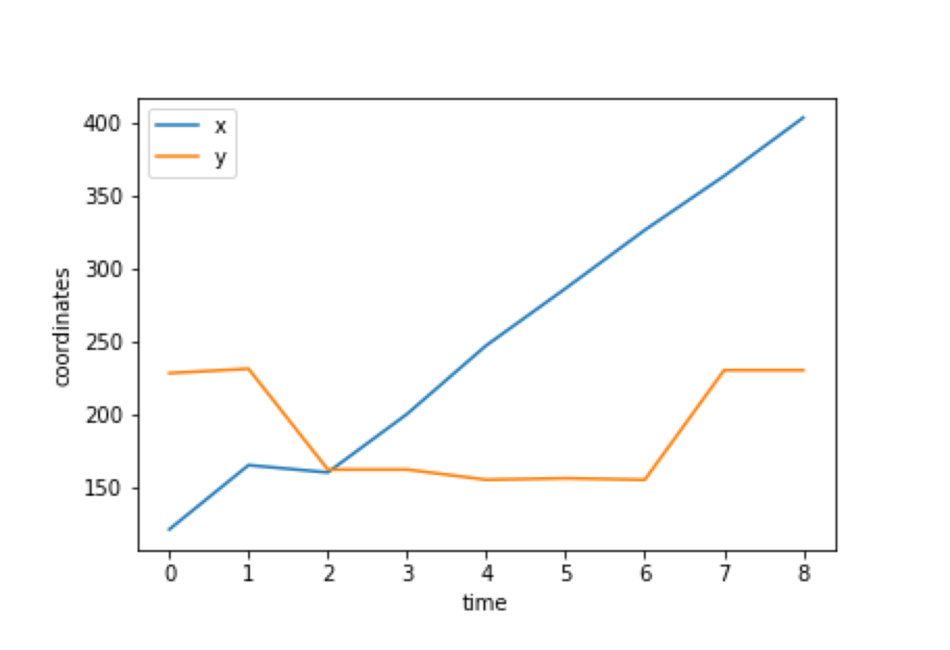
\includegraphics[height=5cm]{b_2_4.eps}
        \subcaption{距離2.4の動作の座標変化}
        \label{b_2_4}
      \end{minipage} &
      \begin{minipage}[t]{0.45\hsize}
        \centering
        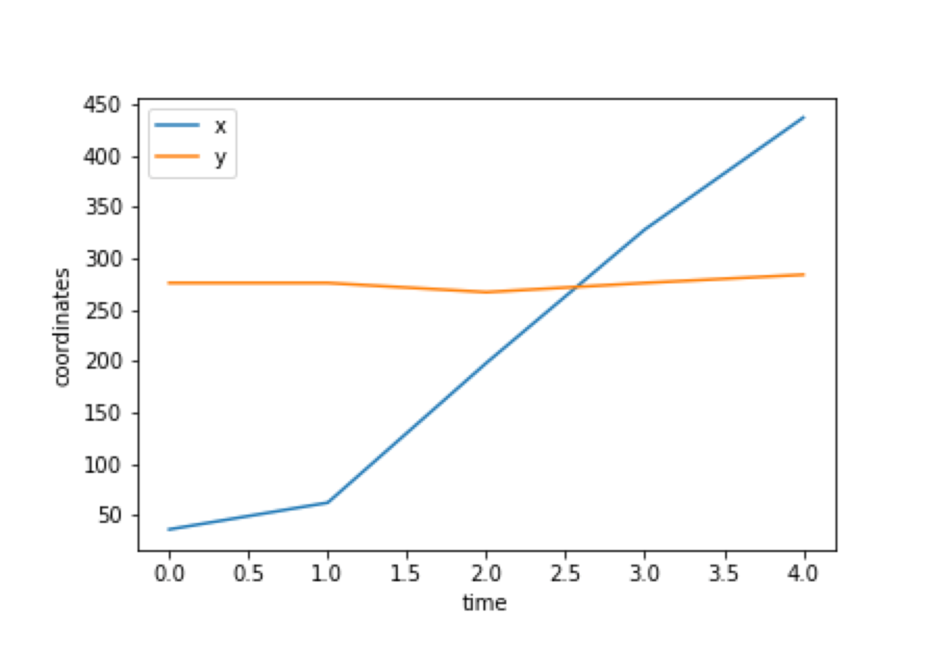
\includegraphics[height=5cm]{b_2_8.eps}
        \subcaption{距離2.8の動作の座標変化}
        \label{b_2_8}
      \end{minipage}
    \end{tabular}
    \caption{入力bのアンケートに提示した動作の例2}
    \label{inputb-ex2}
\end{figure}

\begin{table}[H]
    \caption{入力cのアンケート結果}
    \label{resultc}
    \centering
    \scalebox{0.8}{
    \begin{tabular}{c|c|c|c|c|c|c}
    \hline
     & \multicolumn{4}{c|}{質問1の回答数} & \multicolumn{2}{c}{質問2の回答数} \\
    \hline
    距離 & 1: 類似する & 2: やや類似する & 3: やや類似しない & 4: 類似しない & 1: 実装できる & 2: 実装できない \\
    \hline \hline
    1.7 & 0 & 3 & 0 & 0 & 3 & 0 \\
    \hline
    2.2 & 3 & 0 & 0 & 0 & 3 & 0 \\
    \hline
    2.6 & 0 & 2 & 1 & 0 & 0 & 3 \\
    \hline
    3.0 & 3 & 0 & 0 & 0 & 3 & 0 \\
    \hline
    3.3 & 2 & 1 & 0 & 0 & 3 & 0 \\
    \hline
    3.7 & 2 & 0 & 1 & 0 & 3 & 0 \\
    \hline
    3.8 & 2 & 0 & 1 & 0 & 0 & 3 \\
    \hline
    3.9 & 1 & 1 & 1 & 0 & 3 & 0 \\
    \hline
    4.0 & 1 & 1 & 0 & 1 & 1 & 2 \\
    \hline
    4.1 & 0 & 0 & 0& 3 & 0 & 3 \\
    \hline
    4.3 & 0 & 0 & 0& 3 & 0 & 3 \\
    \hline
    4.4 & 0 & 0 & 0 & 3 & 0 & 3 \\
    \hline
    4.5 & 2 & 1 & 0 & 0 & 3 & 0 \\
    \hline
    4.6 & 0 & 0 & 1 & 2 & 1 & 2 \\
    \hline
    4.7 & 1 & 1 & 1 & 0 & 2 & 1 \\
    \hline
    4.8 & 0 & 0 & 2 & 1 & 2 & 1 \\
    \hline
    4.9 & 1 & 0 & 1 & 0 & 0 & 3 \\
    \hline
    5.0 & 0 & 1 & 2 & 0 & 3 & 0 \\
    \hline
    5.1 & 0 & 0 & 0 & 3 & 0 & 3 \\
    \hline
    5.2 & 0 & 0 & 2 & 1 & 1 & 2 \\
    \hline
    5.3 & 0 & 0 & 0 & 3 & 1 & 2 \\
    \hline
    5.4 & 0 & 0 & 0 & 3 & 0 & 3 \\
    \hline
    5.5 & 1 & 2 & 0 & 0 & 3 & 0 \\
    \hline
    5.6 & 1 & 2 & 0 & 0 & 3 & 0 \\
    \hline
    5.7 & 0 & 1 & 2 & 0 & 2 & 1 \\
    \hline
    5.8 & 0 & 0 & 1 & 2 & 0 & 3 \\
    \hline
    5.9 & 0 & 1 & 2 & 0 & 1 & 2 \\
    \hline
    6.0 & 0 & 0 & 0 & 3 & 0 & 3 \\
    \hline
    6.1 & 0 & 0 & 0 & 3 & 0 & 3 \\
    \hline
    6.2 & 0 & 0 & 0 & 3 & 0 & 3 \\
    \hline
    6.3 & 0 & 0 & 0 & 3 & 0 & 3 \\
    \hline
    6.4 & 0 & 0 & 0 & 3 & 0 & 3 \\
    \hline
    6.5 & 0 & 0 & 0 & 3 & 1 & 2 \\
    \hline
    6.6 & 0 & 0 & 0 & 3 & 0 & 3 \\
    \hline
    6.7 & 0 & 0 & 0 & 3 & 0 & 3 \\
    \hline
    6.8 & 2 & 0 & 1 & 0 & 2 & 1 \\
    \hline
    6.9 & 0 & 0 & 0 & 3 & 0 & 3 \\
    \hline
    \end{tabular}
    }
\end{table} 

\begin{figure}[H]
    \begin{tabular}{cc}
      \begin{minipage}[t]{0.45\hsize}
        \centering
        \includegraphics[height=5cm]{c_1_7.eps}
        \subcaption{距離1.7の動作の座標変化}
        \label{c_1_7}
      \end{minipage} &
      \begin{minipage}[t]{0.45\hsize}
        \centering
        \includegraphics[height=5cm]{c_2_6.eps}
        \subcaption{距離2.6の動作の座標変化}
        \label{c_2_6}
      \end{minipage} \\
   
      \begin{minipage}[t]{0.45\hsize}
        \centering
        \includegraphics[height=5cm]{c_3_3.eps}
        \subcaption{距離3.3の動作の座標変化}
        \label{c_3_3}
      \end{minipage} &
      \begin{minipage}[t]{0.45\hsize}
        \centering
        \includegraphics[height=5cm]{c_3_7.eps}
        \subcaption{距離3.7の動作の座標変化}
        \label{c_3_7}
      \end{minipage} \\
      
      \begin{minipage}[t]{0.45\hsize}
        \centering
        \includegraphics[height=5cm]{c_3_8.eps}
        \subcaption{距離3.8の動作の座標変化}
        \label{c_3_3}
      \end{minipage} &
      \begin{minipage}[t]{0.45\hsize}
        \centering
        \includegraphics[height=5cm]{c_4_0.eps}
        \subcaption{距離4.0の動作の座標変化}
        \label{c_4_0}
      \end{minipage} \\
      
      \begin{minipage}[t]{0.45\hsize}
        \centering
        \includegraphics[height=5cm]{c_4_1.eps}
        \subcaption{距離4.1の動作の座標変化}
        \label{c_4_1}
      \end{minipage} &
      \begin{minipage}[t]{0.45\hsize}
        \centering
        \includegraphics[height=5cm]{c_4_4.eps}
        \subcaption{距離4.4の動作の座標変化}
        \label{c_4_4}
      \end{minipage}
      \end{tabular}
    \caption{入力cのアンケートに提示した動作の例1}
    \label{inputc-ex}
\end{figure}    

\begin{figure}[H]
    \begin{tabular}{cc}
      \begin{minipage}[t]{0.45\hsize}
        \centering
        \includegraphics[height=5cm]{c_4_5.eps}
        \subcaption{距離4.5の動作の座標変化}
        \label{c_4_5}
      \end{minipage} &
      \begin{minipage}[t]{0.45\hsize}
        \centering
        \includegraphics[height=5cm]{c_4_9.eps}
        \subcaption{距離4.9の動作の座標変化}
        \label{c_4_9}
      \end{minipage} \\
   
      \begin{minipage}[t]{0.45\hsize}
        \centering
        \includegraphics[height=5cm]{c_5_5.eps}
        \subcaption{距離5.5の動作の座標変化}
        \label{c_5_5}
      \end{minipage} &
      \begin{minipage}[t]{0.45\hsize}
        \centering
        \includegraphics[height=5cm]{c_5_6.eps}
        \subcaption{距離5.6の動作の座標変化}
        \label{c_5_6}
      \end{minipage} \\
    \end{tabular}
    \caption{入力cのアンケートに提示した動作の例2}
    \label{inputc-ex2}
\end{figure}        

\begin{table}[H]
    \caption{入力dのアンケート結果}
    \label{resultd}
    \centering
    \scalebox{0.8}{
    \begin{tabular}{c|c|c|c|c|c|c}
    \hline
     & \multicolumn{4}{c|}{質問1の回答数} & \multicolumn{2}{c}{質問2の回答数} \\
    \hline
    距離 & 1: 類似する & 2: やや類似する & 3: やや類似しない & 4: 類似しない & 1: 実装できる & 2: 実装できない \\
    \hline \hline
    1.7 & 3 & 0 & 0 & 0 & 3 & 0 \\
    \hline
    3.2 & 0 & 0 & 2 & 1 & 0 & 3 \\
    \hline
    4.3 & 0 & 0 & 1 & 2 & 1 & 2 \\
    \hline
    4.4 & 0 & 2 & 0 & 1 & 3 & 0\\
    \hline
    4.5 & 0 & 0 & 0 & 3 & 1 & 2 \\
    \hline
    4.6 & 0 & 0 & 0 & 3 & 1 & 2 \\
    \hline
    4.7 & 0 & 0 & 0 & 3 & 0 & 3 \\
    \hline
    4.8 & 0 & 0 & 2 & 1 & 0 & 3 \\
    \hline
    5.0 & 0 & 0 & 0& 3 & 0 & 3 \\
    \hline
    5.1 & 0 & 2 & 0& 1 & 3 & 0 \\
    \hline
    5.2 & 0 & 1 & 1& 1 & 3 & 0 \\
    \hline
    5.3 & 0 & 1 & 2 & 0 & 1 & 2 \\
    \hline
    5.4 & 0 & 2 & 0 & 1 & 3 & 0 \\
    \hline
    5.5 & 0 & 2 & 1 & 0 & 2 & 1 \\
    \hline
    5.6 & 0 & 1 & 1 & 1 & 3 & 0 \\
    \hline
    5.9 & 0 & 1 & 1 & 1 & 3 & 0 \\
    \hline
    6.0 & 0 & 0 & 0 & 3 & 1 & 2 \\
    \hline
    6.1 & 0 & 0 & 0 & 3 & 0 & 3 \\
    \hline
    6.2 & 0 & 2 & 0 & 1 & 3 & 0 \\
    \hline
    6.3 & 0 & 0 & 0 & 3 & 1 & 2 \\
    \hline
    6.4 & 0 & 2 & 0 & 1 & 3 & 0 \\
    \hline
    6.5 & 0 & 0 & 0 & 3 & 0 & 3 \\
    \hline
    6.6 & 0 & 1 & 1 & 1 & 1 & 2 \\
    \hline
    6.8 & 0 & 0 & 0 & 3 & 0 & 3 \\
    \hline
    6.9 & 0 & 0 & 0 & 3 & 0 & 3 \\
    \hline
    7.0 & 0 & 0 & 0 & 3 & 0 & 3 \\
    \hline
    7.1 & 0 & 0 & 1 & 2 & 1 & 2 \\
    \hline
    7.2 & 0 & 0 & 0 & 3 & 0 & 3 \\
    \hline
    7.3 & 0 & 2 & 0 & 1 & 1 & 2 \\
    \hline
    7.4 & 0 & 2 & 0 & 1 & 3 & 0 \\
    \hline
    7.5 & 0 & 0 & 0 & 3 & 0 & 3 \\
    \hline
    7.6 & 0 & 0 & 0 & 3 & 1 & 2 \\
    \hline
    7.7 & 0 & 0 & 1 & 2 & 1 & 2 \\
    \hline
    7.8 & 0 & 0 & 0 & 3 & 0 & 3 \\
    \hline
    7.9 & 0 & 0 & 0 & 3 & 1 & 2 \\
    \hline
    \end{tabular}
    }
\end{table} 

\begin{figure}[H]
    \begin{tabular}{cc}
      \begin{minipage}[t]{0.45\hsize}
        \centering
        \includegraphics[height=5cm]{d_1_7.eps}
        \subcaption{距離1.7の動作の座標変化}
        \label{d_1_7}
      \end{minipage} &
      \begin{minipage}[t]{0.45\hsize}
        \centering
        \includegraphics[height=5cm]{d_4_5.eps}
        \subcaption{距離4.5の動作の座標変化}
        \label{d_4_5}
      \end{minipage} \\
   
      \begin{minipage}[t]{0.45\hsize}
        \centering
        \includegraphics[height=5cm]{d_5_1.eps}
        \subcaption{距離5.1の動作の座標変化}
        \label{d_5_1}
      \end{minipage} &
      \begin{minipage}[t]{0.45\hsize}
        \centering
        \includegraphics[height=5cm]{d_5_4.eps}
        \subcaption{距離5.4の動作の座標変化}
        \label{d_5_4}
      \end{minipage} \\
      
      \begin{minipage}[t]{0.45\hsize}
        \centering
        \includegraphics[height=5cm]{d_6_2.eps}
        \subcaption{距離6.2の動作の座標変化}
        \label{d_6_2}
      \end{minipage} &
      \begin{minipage}[t]{0.45\hsize}
        \centering
        \includegraphics[height=5cm]{d_6_4.eps}
        \subcaption{距離6.4の動作の座標変化}
        \label{d_6_4}
      \end{minipage} \\
      
      \end{tabular}
    \caption{入力dのアンケートに提示した動作の例}
    \label{inputd-ex}
\end{figure}

\section{検索評価} 
\label{ranking}     
本研究で提案する検索手法の精度を評価するために,各入力に対する距離算出結果のうち,距離の近い上位20件を用いて
\ref{teisei}節と同様にアンケートを実施した.
検索評価のために,平均逆順位(MRR: Mean Reciprocal Rank)を算出する.
MRRは,ランキング中に初めて正解が出現した順位$rank$の逆数を全ての入力$Q$について平均した
ランキング指標であり,式\ref{mrr}で求められる.
\begin{eqnarray}
    \label{mrr}
    MRR = \frac{1}{|Q|}\sum_{i=1}^{|Q|}\frac{1}{rank_i}
\end{eqnarray}
アンケートの結果から,初めて回答者全員が質問1に対して「1: 類似する」を選択した動作を正解とし,
MRRを算出した結果0.88となった.
入力cのみ正解が出現した順位が2となり,入力a, b, dにおいて正解が出現した順位はいずれも1であった.
MRRの算出結果は0.5を超えており,提案手法による検索において上位に類似動作が出現することが期待できる.

\chapter{考察}
本章では\ref{analysys}章で実施した分析結果から,
動作に基づく検索手法の実用性と,抽出した類似動作のプログラムについて考察する.

\section{動作に基づく検索手法の実用性}

入力aから入力dまで,類似動作を抽出可能な距離は異なる結果となった.
入力a,c,dの類似動作を抽出可能な距離はそれぞれ4.3未満,4.1未満,4.5未満であるのに対し,
入力bは2.2未満と距離が近い結果となった.

入力bにおいて類似動作を抽出可能な距離が近くなった要因を探るために,
回答者全員が類似すると判断した距離0.9の動作1と,回答者全員が類似しないと判断した距離2.2の動作2の
距離算出および図\ref{1-2}に示す座標変化のグラフ作成を行なった.
2つの動作の距離は1.6であり,入力bとの類似動作を抽出可能な距離2.2未満となっている.
図中の横軸は時間(取得したスナップショットの番号)を示し,
縦軸は図\ref{1-2-x}ではx座標,図\ref{1-2-y}ではy座標を示す.
各動作の各点にとって最も距離の近い点が灰色の線で結ばれている.
動作2のスナップショットは左上から右下への直線移動をしているため,
動作2のy座標は値が大きくなっていくと考えたが,
図\ref{1-2-y}から実際にはy座標が動作1と同様に,値が小さくなったあとに
3番目のスナップショットから大きくなっていることがわかる.
スナップショットを確認した結果,スナップショット中でオブジェクトの画像が変更されており,
画像認識の際に取得したオブジェクトの中心座標に変化があることが,
動作の見た目と実際の座標変化に違いが見られた要因であると考えられる.
そのため,座標変化取得のための画像認識を行う際に,
テンプレート画像の中心座標を調整することが必要であることが明らかになった.

\begin{figure}[H]
    \centering
    \begin{minipage}{0.45\linewidth}
        \centering
        \includegraphics[height=5cm]{1-2-x.eps}
        \subcaption{x座標の変化}
        \label{1-2-x}
    \end{minipage}
    \hspace{0.04\columnwidth}
    \begin{minipage}{0.45\linewidth}
        \centering
        \includegraphics[height=5cm]{1-2-y.eps}
        \subcaption{y座標の変化}
        \label{1-2-y}
    \end{minipage}
    \hspace{0.04\columnwidth}
    \caption{動作1と動作2の座標変化グラフ}
    \label{1-2}
\end{figure}

また,入力b,c,dにおいて移動方向は類似するが曲線(直線)移動ではなく
直線(曲線)移動をする動作が見られた要因を探るために,
入力cにおいて回答者全員が類似すると判断した,
入力同様直線移動を行う距離2.2の動作3と,
移動方向は類似するが曲線移動をする距離4.1の動作4の
距離算出および図\ref{3-4}に示す座標変化のグラフ作成を行なった.
2つの動作の距離3.8であり,入力cとの類似動作を抽出可能な距離4.1未満となっている.
図中の横軸は時間(取得したスナップショットの番号)を示し,
縦軸は図\ref{3-4-x}ではx座標,図\ref{3-4-y}ではy座標を示す.
各動作の各点にとって最も距離の近い点が灰色の線で結ばれている.
直線移動を行う動作3は,x座標が変化する際にy座標が変化せず(スナップショット0~6番など),
y座標が変化する際にx座標が変化しない(スナップショット6~10番など)ことが,
曲線移動を行う動作4は,x座標・y座標共に変化し続けていることがグラフから読み取れる.
しかし,値が増加した点同士や減少した点同士で灰色の線が引かれていることから,
値の増減の仕方が類似しており距離が近くなったと考えられる.
直線移動と曲線移動を正しく区別し検索するためには,
より細かい時間で座標変化を取得する必要があると考える.

\begin{figure}[H]
    \centering
    \begin{minipage}{0.45\linewidth}
        \centering
        \includegraphics[height=5cm]{3-4-x.eps}
        \subcaption{x座標の変化}
        \label{3-4-x}
    \end{minipage}
    \hspace{0.04\columnwidth}
    \begin{minipage}{0.45\linewidth}
        \centering
        \includegraphics[height=5cm]{3-4-y.eps}
        \subcaption{y座標の変化}
        \label{3-4-y}
    \end{minipage}
    \hspace{0.04\columnwidth}
    \caption{動作3と動作4の座標変化グラフ}
    \label{3-4}
\end{figure}

本研究では複数の入力における類似動作を抽出可能な距離を明らかにしたが,
入力には無数のパターンが存在するため,全ての入力に対して
類似動作を抽出可能な距離を決定することは不可能である.
また,類似動作を抽出可能な距離以降にも回答者が類似すると判断する動作がいくつか見られた.
これらのことから,検索結果の動作を抽出する距離を一意に定めるのではなく,
\ref{teiryou}のような手法を用いて,
入力と移動方向が異なる動作を抽出する距離をおおまかに求めることが適切である.

動作に基づく検索手法の精度を向上させるためには,画像認識や座標変化を取得する時間間隔といった
検索の前処理における工夫や類似動作を抽出する距離の見直しの必要性が明らかになった.
しかし,\ref{teisei}で実施したアンケート結果から
いずれの入力においても回答者全員が類似すると判断する動作の存在が複数明らかになり,
\ref{ranking}の検索評価の結果からランキング上位に類似動作が出現することが期待できるため,
動作に基づく作品検索は実用性があると考える.

\section{抽出した類似動作のプログラム}
\ref{teisei}で実施したアンケートへの回答時に,複数の実装方法の存在する動作が見られた.
入力bとの距離算出結果が0.9の動作5と,2.1の動作6のプログラムを例に挙げ,
複数の実装方法が検索可能であることの与える学習への影響について考察する.
図\ref{5-6}は動作5と動作6のプログラムを示す.
ただし,「見た目ブロック」といったオブジェクトの動作に直接関係しないブロックは省略している.
図\ref{5-program}に示す動作5のプログラムは,テキストベースのプログラミング言語における
for文に該当する「(引数)回繰り返す」ブロックを用いて,オブジェクトの移動と移動方向の変更を行なっている.
一方,図\ref{6-program}に示す動作6のプログラムは,座標の指定と向きの変更を行うブロックを
必要数並べることで実装している.
動作5のプログラムは,「(引数)回繰り返す」ブロックを用いることで動作6のプログラムよりも可読性が高くなっている.
動作6のプログラムは可読性が低いが,ブロックを1つずつ並べていることから,
どのような順序でオブジェクトが動作しているかを理解しやすくなっている.
動作5,6は,動作は類似するが実装方法に相違点があり,いずれのプログラムにも利点がある.
このことから,実装方法の異なる類似動作を提示することは,
プログラムの実装方法とより良い実装の両方の学習に繋がり,
特に初学者も多く利用しているScratchにおいて有用であると考える.
完全一致による検索であるキーワード検索やプログラム検索でなく,動作に基づく検索をすることによって
類似動作の多様な実装方法を検索することが可能となった.

\begin{figure}
    \centering
    \begin{minipage}{0.45\linewidth}
        \centering
        \includegraphics[height=5cm]{5-program.eps}
        \subcaption{動作5のプログラム}
        \label{5-program}
    \end{minipage}
    \hspace{0.04\columnwidth}
    \begin{minipage}{0.45\linewidth}
        \centering
        \includegraphics[height=20cm]{6-program.eps}
        \subcaption{動作6のプログラム}
        \label{6-program}
    \end{minipage}
    \hspace{0.04\columnwidth}
    \caption{動作5と動作6のプログラム}
    \label{5-6}
\end{figure}


\chapter{おわりに}
本論文では,動作のイメージを入力とするScratch作品の直感的検索手法を提案した.
複数の入力と検索対象動作の距離算出結果に対して分析を行った結果から,次の知見が得られた.

\begin{itemize}
    \item 本研究で提案した手法により,類似動作を検索可能であることが明らかになった.
    さらに,画像認識や座標変化取得の時間間隔といった検索の前処理における工夫や,
    類似動作を抽出する距離の見直しによって,さらなる検索精度の向上が期待できる.
    \item オブジェクトの動作に基づく検索により,類似動作の多様な実装方法を検索可能であることが明らかになった.
    実装方法の異なる類似動作を提示することは,プログラムの実装方法とより良い実装の両方の学習に繋がり,
    特に初学者も多く利用しているScratchにおいて有用である.
\end{itemize}

本論文で提案した手法により,
ユーザのイメージする動作から多様な実装方法の作品を容易に検索することができるため,
他者の作品を参照することによる実装方法学習の支援を期待する.
さらに手法を改善することによって,より精度の高い作品検索の実現を期待する.


%%%%%%%%%%%%%%%%%%%%%%%%%%%%%%%%%%%%%%%%%%%%%%%%%%%%%%%%%%%%%%%%%%%%%%%%

%%
%% 謝辞
%%
 \begin{acknowledgements}
    本研究を進めるにあたり,多くの方々に御指導,御協力,御支援を賜りました.
    ここに御世話になった方々への感謝の意を記させて頂きました.
    
    はじめに,指導教員である和歌山大学システム工学部伊原彰紀講師に対し,厚く御礼申し上げます.
    研究室配属以降,研究の進め方から,論文の執筆,プレゼンテーションの方法,礼儀,研究の面白さなど,
    多くの御指導をして頂きました.特に学会発表などで,様々な研究者と交流する機会を数多く与えて頂き,
    自分の知見を広げることができました.先生のご尽力に敬意を表し,心より感謝致します.
    
    和歌山大学ソーシャルソフトウェア工学研究室の方々には,研究活動に対する多大な御協力,
    御助言を頂きました.研究活動だけでなく,大学生活において大変お世話になりました.
    また,日々切磋琢磨し合う同期の仲間がいたことは,研究活動を進める上で支えとなりました.
    心より感謝致します.
    
    最後になりましたが,研究活動を進めるにあたって支えてくださった家族に対し,心より深く感謝致します.
 \end{acknowledgements}

%%%%%%%%%%%%%%%%%%%%%%%%%%%%%%%%%%%%%%%%%%%%%%%%%%%%%%%%%%%%%%%%%%%%%%%%

%%
%% 参考文献
%%
\begin{thebibliography}{99}

\bibitem{spfa}
 Mitchel Resnick, John Maloney, Andr\'{e}s Monroy-Hern\'{a}ndez, Natalie Rusk, Evelyn Eastmond, Karen Brennan, 
    Amon Millner, Eric Rosenbaum, Jay Saul Silver, Brian S Silverman, Yasmin Bettina Kafai,
 Scratch: Programming for all,
 Communications of the ACM, Vol.52, No.11, pp.60-67, 2009.

\bibitem{behavior}
 Sheela Surisetty, Catherine Law, Chris Scaffidi, 
 Behavior-based clustering of visual code,
 Proceedings of IEEE Symposium on Visual Languages and Human-Centric Computing, pp.261-269, 2015.

\bibitem{wild}
    Aniket Dahotre, Yan Zhang, Christopher Scaffidi,
    A qualitative study of animation programming in the wild,
    ESEM'10: Proceedings of the 2010 ACM-IEEE International Symposium on Empirical Software Engineering and Measurement,
    No.29, pp.1-10, 2010.
    
\bibitem{blocktotext}
    David Weintrop, Uri Wilensky,
    Comparing block-based and text-based programming in high school computer science classrooms,
    ACM Transactions on Computing Education, Vol.18, No.1, pp 1-25, 2018.
    
\bibitem{blockandbeyond}
    David Bau, Jeff Gray, Caitlin Kelleher, Josh Sheldon, Franklyn Turbak,
    Learnable programming: blocks and beyond,
    Communications of the ACM, Vol.60, No.6, pp.72-80, 2017. 

\bibitem{codesearch}
    Susan Elliott Sim, Medha Umarji, Sukanya Ratanotayanon, Cristina V. Lopes,
    How Well Do Search Engines Support Code Retrieval on the Web?,
    ACM Transactions on Software Engineering and Methodology, Vol.21, No.1, pp.1-25, 2011.

\bibitem{sift}
 David G. Lowe.,
 Distinctive Image Features from Scale-Invariant Keypoints,
 International Journal of Computer Vision, Vol.60, pp.91-110, 2004.

\bibitem{dataset}
    Efthimia Aivaloglou, Felienne Hermans, Jes\'{u}s Moreno-Le\'{o}n, Gregorio Robles,
    A dataset of scratch programs: scraped, shaped and scored,
    Proceeding of the 14th International Conference on Mining Software Repositories, pp.511-514, 2017.
 
\end{thebibliography}

\chapter*{対外発表}
\begin{enumerate}
    \item 福地ユキ,伊原彰紀,山本豪志朗,橋谷直樹:
    オブジェクト操作入力に基づくビジュアルプログラミング作品検出の試み,
    情報処理学会 第83回全国大会 講演論文集,pp.265-266.2021.
    \item 福地ユキ,伊原彰紀,山本豪志朗,橋谷直樹:
    ビジュアルプログラミング作品検索のためのオブジェクト操作データの時系列解析,
    2021年度 情報処理学会関西支部 支部大会 講演論文集,2021.
    \item 福地ユキ,伊原彰紀,山本豪志朗,橋谷直樹:
    オブジェクト動作経路の時系列解析に基づくビジュアルプログラム作品検索の試み,
    第28回ソフトウェア工学の基礎ワークショップ(FOSE2021) デモ・ポスター発表,2021.
\end{enumerate}

%%%%%%%%%%%%%%%%%%%%%%%%%%%%%%%%%%%%%%%%%%%%%%%%%%%%%%%%%%%%%%%%%%%%%%%%

%%
%% 付録
%%
% \appendix
% 
% \chapter{サンプルプログラム}
% 
% プログラムリストや実行結果など,本論を補足する上で必要と思われるものが
% あれば付録として付ける.
% 
% {
% \footnotesize
% \begin{verbatim}
% #include <stdio.h>
% int main(void)
% {
%     printf("Hello, World!\n");
%     return 0;
% }
% \end{verbatim}
% }

%%%%%%%%%%%%%%%%%%%%%%%%%%%%%%%%%%%%%%%%%%%%%%%%%%%%%%%%%%%%%%%%%%%%%%%%

\end{document}
